\documentclass[a4paper,12pt]{extarticle}
\usepackage{geometry}
\usepackage[T1]{fontenc}
\usepackage[utf8]{inputenc}
\usepackage[english,russian]{babel}
\usepackage{amsmath}
\usepackage{amsthm}
\usepackage{amssymb}
\usepackage{fancyhdr}
\usepackage{setspace}
\usepackage{graphicx}
\usepackage{colortbl}
\usepackage{tikz}
\usepackage{pgf}
\usepackage{subcaption}
\usepackage{listings}
\usepackage{indentfirst}
\usepackage[
backend=biber,
style=numeric,
maxbibnames=99
]{biblatex}
\addbibresource{refc.bib}
\usepackage[colorlinks,citecolor=blue,linkcolor=blue,bookmarks=false,hypertexnames=true, urlcolor=blue]{hyperref} 
\usepackage{indentfirst}
\usepackage{mathtools}
\usepackage{booktabs}
\usepackage[flushleft]{threeparttable}
\usepackage{tablefootnote}

\usepackage{chngcntr}
\counterwithin{table}{section}
\counterwithin{figure}{section}

\graphicspath{{graphics/}}%путь к рисункам

\makeatletter
% \renewcommand{\@biblabel}[1]{#1.} % Заменяем библиографию с квадратных скобок на точку:
\makeatother

\geometry{left=2.5cm}% левое поле
\geometry{right=1.0cm}% правое поле
\geometry{top=2.0cm}% верхнее поле
\geometry{bottom=2.0cm}% нижнее поле
\setlength{\parindent}{1.25cm}
\renewcommand{\baselinestretch}{1.5} % междустрочный интервал


\newcommand{\bibref}[3]{\hyperlink{#1}{#2 (#3)}} % biblabel, authors, year
\addto\captionsrussian{\def\refname{Список литературы (или источников)}} 

\renewcommand{\theenumi}{\arabic{enumi}}% Меняем везде перечисления на цифра.цифра
\renewcommand{\labelenumi}{\arabic{enumi}}% Меняем везде перечисления на цифра.цифра
\renewcommand{\theenumii}{.\arabic{enumii}}% Меняем везде перечисления на цифра.цифра
\renewcommand{\labelenumii}{\arabic{enumi}.\arabic{enumii}.}% Меняем везде перечисления на цифра.цифра
\renewcommand{\theenumiii}{.\arabic{enumiii}}% Меняем везде перечисления на цифра.цифра
\renewcommand{\labelenumiii}{\arabic{enumi}.\arabic{enumii}.\arabic{enumiii}.}% Меняем везде перечисления на цифра.цифра

\begin{document}
\input{title_kr}% это титульный лист - выберите подходящий вам из имеющихся в проекте вариантов (kr - курсовая работа у 3 курса, vkr - выпускная квалификационная работа у 4 курса)
\newpage
\setcounter{page}{2}

{
	\hypersetup{linkcolor=black}
	\tableofcontents
}
\newpage

\section*{Аннотация}

\addcontentsline{toc}{section}{Аннотация}

Данная работа посвящена задаче предсказания временных связей (temporal link prediction) в крупномасштабном транзакционном графе криптовалюты Bitcoin. В качестве данных используется открытый датасет ORBITAAL, охватывающий историю транзакций с 2009 по 2021~год; для экспериментов выбраны первые 10\% рёбер трёхмесячного периода, что соответствует более 6~миллионам транзакций между 2.6~миллионами кошельков.

В рамках работы реализованы и сравнены более десяти методов предсказания связей: структурные эвристики (Common Neighbors, Adamic--Adar, Jaccard, Preferential Attachment), классические алгоритмы машинного обучения (Logistic Regression, Random Forest, CatBoost), нейросетевая модель CN+MLP, а также современные темпоральные GNN-архитектуры (EAGLE, GraphMixer, GLFormer, DyGFormer). Центральным результатом является неожиданное превосходство структурных методов над нейросетевыми: метод Common Neighbors достигает тестового MRR~=~0.64, опережая все протестированные GNN-архитектуры. Аблационное исследование модели CN+MLP показало, что расширение признакового пространства сверх единственного признака не улучшает, а ухудшает качество.

Помимо экспериментального исследования, разработана Python-библиотека \\ \texttt{payment-graph-forecasting}, предоставляющая единый воспроизводимый конвейер для обучения и оценки моделей на темпоральных платёжных графах. Реализован CUDA-модуль темпорального семплирования и вычисления Common Neighbors, обеспечивающий ускорение до 180~раз на синтетических бенчмарках и двукратное сокращение времени обучения DyGFormer на реальных данных.

\section*{Список ключевых слов}

\addcontentsline{toc}{section}{Список ключевых слов}

temporal link prediction, транзакционные графы, Bitcoin, Common Neighbors, графовые нейронные сети, машинное обучение, динамические графы, CUDA-ускорение, финансовая аналитика, link prediction

\newpage

\section*{Введение}

\addcontentsline{toc}{section}{Введение}

Современные платёжные системы генерируют огромные объёмы транзакционных данных, которые естественным образом представляются в виде графов: узлы соответствуют участникам системы (пользователям, организациям, кошелькам), а рёбра~--- финансовым взаимодействиям между ними. Анализ структуры и динамики подобных графов представляет значительный интерес как для академического сообщества, так и для прикладных задач в области финансовых технологий.

Среди открытых финансовых данных Bitcoin стоит отдельно — это первая и самая популярная криптовалюта, все транзакции которой видны всем желающим с 2009 года. На этом графе транзакций удобно изучать большие финансовые сети: сотни миллионов узлов, миллиарды рёбер, и всё это постоянно растёт. Но у таких графов есть своя специфика, которая отличает их от стандартных датасетов: граф очень разреженный, степени узлов распределены по степенному закону, никаких готовых признаков нет, и одни и те же адреса нередко взаимодействуют снова и снова.

\paragraph{Постановка задачи.}
Данная работа сосредоточена на задаче предсказания временных связей (temporal link prediction): по истории транзакций, наблюдавшихся до момента $t$, необходимо оценить вероятность появления транзакции $(s, d, t)$ между кошельком-источником $s$ и кошельком-назначением $d$. Эта задача является фундаментальной в анализе графов и имеет прямые прикладные применения: выявление мошеннических операций, прогнозирование транзакционной активности, анализ рыночных трендов и стратегическое планирование в финансовых организациях.

\paragraph{Актуальность и новизна.}
Методы предсказания связей на темпоральных графах активно развиваются, но большинство работ проверяют их на небольших социальных или биологических сетях. На реальных крупных финансовых данных современные GNN-архитектуры тестировали значительно реже. Эта работа закрывает пробел: мы систематически сравниваем больше десяти методов — от классических структурных эвристик до современных темпоральных нейросетей — на датасете, который превосходит стандартные бенчмарки на 1–4 порядка по числу узлов и рёбер.

\paragraph{Основные результаты.}
Главный неожиданный результат: структурный метод Common Neighbors (CN), который не требует обучения и смотрит исключительно на топологию графа, обошёл все протестированные нейросетевые модели по метрике MRR ($\text{MRR}_\text{CN} = 0.64$ против $\text{MRR}_\text{EAGLE} = 0.46$ и $\text{MRR}_\text{DyGFormer} = 0.40$). Похоже, в реальных финансовых сетях структурная близость узлов куда лучше предсказывает будущие рёбра, чем темпоральные паттерны, на которых специализируются GNN. Аблационное исследование CN+MLP это подтвердило: добавление любых дополнительных признаков к единственному структурному дескриптору cn\_uu результат не улучшает, а стабильно ухудшает.

Помимо экспериментального сравнения, в рамках проекта разработана Python-библиотека \texttt{payment-graph-forecasting}~--- воспроизводимый конвейер для обучения, оценки и анализа моделей на темпоральных платёжных графах с единым API, типизированными YAML-конфигурациями и автоматическими тестами. Для ускорения вычислительно дорогостоящих операций (темпоральное семплирование соседей и вычисление Common Neighbors) реализован CUDA-модуль с тремя взаимозаменяемыми backend'ами (Python, C++, CUDA), обеспечивающий ускорение до 180~раз на синтетических бенчмарках. Перенос этапа подготовки батча на GPU сокращает время одной эпохи обучения DyGFormer вдвое~--- с~55 до~27.5~минут~--- на реальных данных.

\paragraph{Структура работы.}
Работа организована следующим образом. Раздел «Обзор литературы» рассматривает существующие подходы к предсказанию связей в транзакционных графах и обзор используемых библиотек. Раздел «Задача» содержит формальную постановку задачи, описание метрик, стратегий семплирования и используемого датасета. Раздел «Модели» описывает все сравниваемые методы~--- от структурных эвристик до темпоральных GNN. Раздел «Эксперименты» представляет результаты сравнительного анализа и аблационного исследования CN+MLP. Раздел «Библиотека» описывает архитектуру и функциональность разработанной программной системы. Раздел «CUDA» описывает реализованные вычислительные ускорения.

\paragraph{Распределение задач в команде.}
Проект выполнялся командой из трёх человек.

\textbf{Кречетов Роман Константинович}: обзор научной литературы по методам прогнозирования связей на транзакционных графах; определение направления исследования и выбор методов; реализация и тестирование структурных baseline-методов (CN, AA, Jaccard, PA); выбор и адаптация архитектур нейронных сетей; проведение экспериментов и аблационного исследования CN+MLP; сравнительный анализ результатов.

\textbf{Романюков Егор Сергеевич}: исследование открытых источников платёжных данных и выбор датасета; предобработка данных и формирование рабочей выборки; анализ структурных свойств графа; реализация признакового описания узлов; обучение и оценка классических моделей машинного обучения (Logistic Regression, Random Forest, CatBoost, CN+MLP); формулировка и проверка гипотез по результатам экспериментов.

\textbf{Шеин Илья Антонович}: проектирование и реализация библиотеки \texttt{payment-graph-forecasting}; развёртывание вычислительной инфраструктуры; реализация CUDA-модуля темпорального семплирования и Common Neighbors; интеграция ускоренного пути в обучающий pipeline DyGFormer; документирование библиотеки и написание автоматических тестов.

\newpage

\section*{Обзор литературы}

\addcontentsline{toc}{section}{Обзор литературы}

\subsection*{Обзор работ по прогнозированию транзакционных графов}
\addcontentsline{toc}{subsection}{Обзор работ про транзакции}

Прогнозирование динамики транзакционных графов исследуется в нескольких постановках задач, которые существенно различаются по типу целевой переменной, сложности разметки и методологической зрелости.

\paragraph{Классификация задач.}
В литературе выделяют следующие основные направления.

\textbf{Link prediction (предсказание рёбер)} --- прогноз появления новых транзакционных связей между узлами. Wei et al.~\cite{wei2022bitcoin} решают задачу прогнозирования транзакций в Bitcoin-сети, строя два графа --- на основе достижимости с временным затуханием и на основе паттернов сумм --- и обучая DNN на их конкатенации; достигнутое улучшение составляет $+50\%$ по сравнению со статическим бенчмарком. Tang et al.~\cite{tang2023nft} анализируют NFT-граф Ethereum через ежедневные срезы и сравнивают несколько динамических GNN (GCRN, Roland, DynGraph2Vec), показывая, что мелкая дискретизация (день против месяца) существенно улучшает AUC. Wang et al.~\cite{wang2023exgraph} создают большой датасет EX-Graph (Ethereum + off-chain связи) и демонстрируют, что добавление внегрупповых признаков улучшает предсказание транзакций.

\textbf{Flow/weight prediction (прогноз весов рёбер)} --- оценка объёма платежей на существующих или новых связях. Takahashi et al.~\cite{takahashi2024flow} разбивают задачу на два подзадачи: прогноз соотношения потоков и суммарного объёма, используя GNN с временным само-вниманием; модель проверяется на криптовалютных и банковских данных. По сути это регрессия с числовыми метками, которые сильно зашумлены.

\textbf{Anomaly detection / AML (обнаружение аномалий)} --- выявление мошеннических транзакций или подозрительных узлов. Gounoue et al.~\cite{gounoue2025temptrag} предлагают TeMP-TraG с темпоральным message passing, где недавние транзакции получают больший вес, и показывают прирост F1 по сравнению с классическими GNN. Cheng et al.~\cite{cheng2024gnn} в своём обзоре разбирают более 100 работ по GNN для финансового фрода и фиксируют их стабильное превосходство над традиционными методами. Главная сложность задачи --- размеченные данные: их мало, и разметка часто субъективна.

\textbf{Прогноз агрегированных временных рядов} --- предсказание суммарных метрик (комиссии, объёмы) без явного учёта структуры графа. Ma et al.~\cite{ma2025fees} сравнивают SARIMAX, Prophet и Temporal Fusion Transformer на данных о комиссиях Bitcoin и показывают, что классический SARIMAX при ограниченном объёме данных обходит сложные нейросетевые методы. Задача не опирается на структуру сети --- это одновременно и её простота, и её главное ограничение.

\paragraph{Сравнение постановок и обоснование выбора temporal link prediction.}
В таблице~\ref{tab:task_comparison} представлено сравнение постановок по ключевым критериям.

\begin{table}[ht]
    \caption{Сравнение постановок задач прогнозирования транзакций}
    \label{tab:task_comparison}
    \footnotesize
    \centering
    \begin{tabular}{lcccc}
        \toprule
        Задача & Метки доступны & Сложность разметки & Учёт структуры & Метрики \\
        \midrule
        Link prediction          & да (из данных) & минимальная & да & AUC, MRR, H@K \\
        Flow/weight prediction   & частично       & средняя (шум) & да & MAE, RMSE \\
        Anomaly detection        & редко          & высокая       & да & F1, F2 \\
        Прогноз временных рядов  & да             & минимальная   & нет & RMSE, MAPE \\
        \bottomrule
    \end{tabular}
\end{table}

Temporal link prediction является оптимальным выбором по нескольким причинам. Во-первых, целевые метки (факт появления транзакции между двумя узлами) естественно доступны из исторических данных без дополнительной разметки. Во-вторых, для этой задачи выработаны устоявшиеся метрики (MRR, Hits@K), хорошо работающие на разреженных динамических графах~\cite{poursafaei2022towards}. В-третьих, постановка напрямую нацелена на прогнозирование сетевой структуры потока платежей, а не на агрегированные показатели. Альтернативы уступают по одному или нескольким критериям: flow prediction требует точных числовых меток со значительным шумом; anomaly detection страдает от редкости и субъективности меток мошенничества; прогноз временных рядов игнорирует топологию графа. В связи с этим в данной работе в качестве основной задачи выбрано \emph{temporal link prediction}.

\subsection*{Обзор моделей для прогнозирования}
\addcontentsline{toc}{subsection}{Обзор моделей для прогнозирования}

Методы предсказания связей в динамических графах делятся на несколько классов~\cite{kazemi2020representation, xiong2026survey}.

\paragraph{Структурные эвристики.}
Классические меры схожести --- Common Neighbours (CN), Adamic--Adar (AA), Jaccard, Preferential Attachment (PA)~\cite{liben2007link, adamic2003friends, barabasi1999emergence} --- работают со статическим графом, не учитывают время и не требуют обучения. Они вычислительно дёшевы и хорошо интерпретируемы, но ограничены структурой первого порядка.

\paragraph{Классические методы машинного обучения.}
Логистическая регрессия, случайные леса~\cite{breiman2001random} и градиентный бустинг (CatBoost~\cite{prokhorenkova2018catboost}) обучаются на вручную сконструированных признаках пар узлов. Они сильнее эвристик за счёт использования атрибутивной информации, но также не моделируют темпоральность явно.

\paragraph{Методы на основе графовых эмбеддингов.}
Node2Vec, DeepWalk и GCN работают со статическим графом. Для динамических графов разработаны DynGEM и DynGraph2Vec~\cite{goyal2018dynamgem}, использующие автоэнкодеры и RNN на серии срезов, а также CTDNE~\cite{nguyen2018continuous} с непрерывными случайными блужданиями и временными метками.

\paragraph{Временные графовые нейронные сети (Temporal GNN).}
Это наиболее развитый на сегодня класс методов. \textbf{EvolveGCN}~\cite{pareja2019evolvegcn} эволюционирует параметры GCN через RNN, работая на дискретных снимках. \textbf{TGAT}~\cite{xu2020inductive} вводит функциональное кодирование времени в механизм само-внимания, обеспечивая индуктивность и учёт непрерывных временных меток. \textbf{TGN}~\cite{rossi2020temporal} добавляет к GNN явный модуль памяти для каждого узла, обновляемый через GRU, что позволяет захватывать долгосрочные зависимости и достигает SOTA на ряде бенчмарков. \textbf{DyRep}~\cite{trivedi2019representation} моделирует граф через временные точечные процессы, прогнозируя не только наличие ребра, но и время его появления. \textbf{GraphMixer}~\cite{cong2023graphmixer} демонстрирует, что конкурентоспособного качества можно достичь без механизма внимания --- только на MLP и mean-pooling. \textbf{GLFormer}~\cite{liao2024glformer} заменяет self-attention на адаптивную агрегацию токенов с экспоненциально расширяющимся рецептивным полем, снижая сложность с $O(N^2)$ до $O(N \sum_l K_l)$. \textbf{DyGFormer}~\cite{yu2023towards} формирует патчи из исторических последовательностей обоих узлов и обрабатывает их трансформером с механизмом кодирования совместной встречаемости соседей (NCoE).

\paragraph{Обоснование выбора моделей в данной работе.}
В качестве базовых решений выбраны структурные эвристики (CN, AA, Jaccard, PA) и классические модели машинного обучения (CN+MLP, LogReg, RF, CatBoost). Они образуют сильный нижний порог: как показано в~\cite{poursafaei2022towards}, на ряде реальных датасетов простые эвристики неожиданно конкурентоспособны по сравнению со сложными Temporal GNN.

В качестве глубоких моделей выбраны \textbf{EAGLE}, \textbf{GraphMixer}, \textbf{GLFormer} и \textbf{DyGFormer}. Этот набор репрезентативен по нескольким осям. По архитектуре он охватывает лёгкие агрегирующие методы без обучаемого внимания (EAGLE, GraphMixer) и Transformer-подобные архитектуры (GLFormer, DyGFormer). По вычислительной сложности --- от почти линейных (EAGLE, GraphMixer) до квадратичных в длине истории (DyGFormer). По способу учёта времени --- от адаптивных весов на основе временных интервалов (EAGLE, GLFormer) до явного патчинга и кодирования временных смещений (DyGFormer, GraphMixer). Как отмечается в обзорных работах~\cite{xiong2026survey}, не существует единой универсальной архитектуры для всех типов графов и задач, поэтому одновременное рассмотрение нескольких разнородных подходов позволяет получить более полную картину.

\subsection*{Обзор библиотек}
\addcontentsline{toc}{subsection}{Обзор библиотек}

Прежде чем перейти к описанию нашего подхода, стоит обозначить, на фоне чего он
существует. Задача обучения на динамических графах активно развивается последние
несколько лет, и за это время сложился ряд устойчивых решений. Наиболее
распространённые из них — PyTorch Geometric Temporal и базовый PyG — ориентированы
либо на дискретные временные снимки (один граф на момент времени)
\cite{pytorch_geometric_temporal}, либо предоставляют низкоуровневые
примитивы вроде \texttt{TemporalData}, из которых пользователь сам собирает
нужный пайплайн \cite{pytorch_temporaldata_docs}. DGL занимает похожую нишу:
мощный и гибкий фреймворк общего назначения, но без специализированной поддержки
темпоральности «из коробки» \cite{dgl}. Более специализированные решения — TGL от
Amazon и STM-Graph — решают конкретные промышленные задачи (сверхкрупные графы,
городской трафик) и плохо обобщаются за пределы своей ниши \cite{tgl_amazon,stm_graph}.
На этом фоне выделяется DyGLib — библиотека, созданная авторами DyGFormer и
сосредоточённая именно на непрерывных событийных графах: тех, где данные задаются
потоком взаимодействий \texttt{(src, dst, timestamp)}
\cite{dyglib_openreview,dyglib_github}. Это в точности наш формат
\texttt{stream\_graph}. DyGLib предлагает единый воспроизводимый конвейер,
охватывающий ряд современных методов и датасетов, и при этом
аккуратно закрывает как задачи предсказания связей, так и задачи на уровне
узлов \cite{dyglib_openreview,dyglib_github}. Немаловажно, что авторы намеренно
выявляли и исправляли методологические несоответствия в предшествующих
реализациях — то есть библиотека изначально проектировалась как честный инструмент
сравнения, а не просто витрина одной модели \cite{dyglib_openreview,dyglib_github}.
Именно поэтому DyGLib является наиболее естественным ориентиром для нашей работы:
она свежая, методологически строгая и работает с тем же типом данных. Именно поэтому в
дальнейшем в качестве основного ориентира для сравнения мы будем использовать библиотеку DyGLib.

DyGLib представляет собой сильное исследовательское решение для задач обучения на непрерывных темпоральных графах. К его достоинствам относятся единый
  экспериментальный конвейер, поддержка нескольких стандартных задач, прежде всего temporal link prediction и node classification, набор распространённых стратегий
  негативного семплирования, а также включение ряда известных моделей, охватывающих важную часть классической литературы по dynamic graph learning
  \cite{dyglib_openreview,dyglib_github}. В этом смысле библиотека удобна как воспроизводимый benchmark framework. Вместе с тем DyGLib в большей степени
  ориентирован на оффлайн-эксперименты на заранее подготовленных датасетах, чем на роль универсальной библиотечной платформы: работа с данными привязана к
  фиксированному формату предобработанных CSV/NPY-файлов, а добавление новых моделей и сценариев требует прямого изменения тренировочных и оценочных скриптов
  \cite{dyglib_github}. Кроме того, основной набор реализованных в DyGLib методов сосредоточен главным образом на уже устоявшихся архитектурах, поэтому покрытие
  более новых направлений остаётся ограниченным \cite{dyglib_github}. Наконец, в доступной реализации DyGLib вспомогательные вычисления, связанные с выборкой
  исторических соседей и частью процедур негативного семплирования, выполняются на стороне CPU средствами Python/NumPy; отдельного бэкенда на C++ или CUDA для
  этих этапов в библиотеке не представлено \cite{dyglib_github}. Из-за этого на крупных графах и при длинной истории взаимодействий ускорение со стороны GPU
  ограничивается тем, что заметная доля времени уходит на предварительную CPU-обработку данных.

\newpage

\section{Задача}

\subsection{Постановка задачи}

Рассматривается задача предсказания временных связей (temporal link prediction) в динамическом направленном графе \cite{kazemi2020representation, longa2023graph}. Динамический граф представляется как поток событий (stream graph) $\mathcal{G} = (\mathcal{V}, \mathcal{E})$, где $\mathcal{V}$ — конечное множество узлов, а $\mathcal{E} = \{(s_i, d_i, t_i)\}_{i=1}^{|\mathcal{E}|}$ — хронологически упорядоченное множество направленных рёбер с временными метками: $t_1 \leq t_2 \leq \dots \leq t_{|\mathcal{E}|}$. Каждое ребро $(s, d, t) \in \mathcal{E}$ означает взаимодействие от узла-источника $s \in \mathcal{V}$ к узлу-назначению $d \in \mathcal{V}$ в момент времени $t \in \mathbb{R}_{+}$.

Задача состоит в следующем: дан граф $\mathcal{G}_{<t} = (\mathcal{V}, \{(s_i, d_i, t_i) \in \mathcal{E} \mid t_i < t\})$, содержащий все взаимодействия, предшествующие моменту времени $t$; требуется оценить вероятность $P(s, d, t \mid \mathcal{G}_{<t})$ появления нового ребра $(s, d, t)$ между заданной парой узлов $(s, d)$.

Для обучения и оценки качества модели рёбра разбиваются на три непересекающихся непрерывных временных интервала. Пусть хронологически упорядоченные рёбра пронумерованы от $1$ до $|\mathcal{E}|$. Тогда:
\begin{itemize}
    \item \textbf{Обучающая выборка} $\mathcal{E}_{\text{train}}$: первые 70\% рёбер по временному порядку, то есть $\mathcal{E}_{\text{train}} = \{(s_i, d_i, t_i) \mid i \leq \lfloor 0.7 \cdot |\mathcal{E}| \rfloor\}$.
    \item \textbf{Валидационная выборка} $\mathcal{E}_{\text{val}}$: следующие 15\% рёбер.
    \item \textbf{Тестовая выборка} $\mathcal{E}_{\text{test}}$: последние 15\% рёбер.
\end{itemize}
Такое разбиение по временному принципу (temporal split) исключает любую утечку данных из будущего в прошлое \cite{poursafaei2022towards}: модель в момент оценки на тестовой выборке имеет доступ только к рёбрам из $\mathcal{E}_{\text{train}}$ и $\mathcal{E}_{\text{val}}$.

Помимо транзакционных рёбер, узлы и рёбра могут быть снабжены атрибутными признаками. В рамках данной работы признаки ребра кодируют объём транзакции в единицах биткоина. Функция узловых признаков $\mathbf{x}_v(t) \in \mathbb{R}^{d_v}$ представляет статические или динамические свойства узла $v$, вычисляемые на основе $\mathcal{E}_{\text{train}}$ (см. раздел о признаках). Таким образом, задача предсказания связей формально сводится к задаче бинарной классификации пар узлов $(s, d)$ при заданном моменте времени $t$: модель должна отличить реальное ребро от заданного множества отрицательных примеров \cite{xu2020inductive}.

\subsection{Семплирование негативных рёбер}

При оценке модели на задаче предсказания связей для каждого истинного (положительного) ребра $(s, d, t) \in \mathcal{E}_{\text{eval}}$ необходимо сформировать набор отрицательных рёбер — несуществующих взаимодействий, которые модель должна отличить от реального. Качество и репрезентативность этого набора существенно влияют на оценки метрик \cite{poursafaei2022towards}.

Различают три основных стратегии семплирования негативных рёбер:

\begin{enumerate}
    \item \textbf{Случайное семплирование (random negatives, RND).} Для каждого позитивного ребра $(s, d, t)$ случайным образом сэмплируется узел $d' \in \mathcal{V}$, $d' \neq d$, и формируется отрицательный пример $(s, d', t)$. Аналогично можно фиксировать $d$ и случайным образом выбирать источник $s'$. Данная стратегия является наиболее распространённой, однако считается чрезмерно простой: большинство случайных пар узлов никогда не взаимодействовали, и модель может легко их отсеять.

    \item \textbf{Исторически обоснованные негативы (historical negatives, HIST).} Отрицательные примеры выбираются из пар узлов, которые взаимодействовали в прошлом (до момента $t$), но не являются истинным ребром в данный момент. Такая стратегия существенно усложняет задачу, поскольку модель должна отличать реальное взаимодействие от схожих по структуре исторических.

    \item \textbf{Индуктивные негативы (inductive negatives, IND).} Отрицательные примеры включают пары узлов, хотя бы один из которых не встречался в обучающей выборке. Данная стратегия проверяет способность модели обобщаться на новые (unseen) узлы, что особенно важно в индуктивном сценарии.
\end{enumerate}

В данной работе используется стратегия случайного семплирования негативных рёбер с фиксированным узлом-источником: для каждого позитивного ребра $(s, d, t)$ случайным образом выбирается один отрицательный узел назначения $d'$, формируя пару $(s, d', t)$.

\subsection{Стратегия формирования кандидатов}

При оценке моделей по метрикам ранжирования для каждого ребра из оценочной выборки формируется список кандидатов, состоящий из истинного ребра и $N_{\text{neg}}$ отрицательных. Модель ранжирует кандидатов по предсказанной вероятности взаимодействия, и оценивается позиция истинного ребра в этом ранжировании.

Различают два основных подхода к формированию кандидатов:

\begin{itemize}
    \item \textbf{Полный список кандидатов (full candidate set).} В качестве кандидатов рассматриваются все узлы $\mathcal{V}$, кроме истинного назначения. Метрики, вычисленные на полном списке кандидатов, отражают реальное качество ранжирования, однако вычислительно затратны для больших графов ($|\mathcal{V}|$ может составлять миллионы узлов).

    \item \textbf{Выборочный список кандидатов (sampled candidate set).} Для каждого позитивного ребра $(s, d, t)$ случайным образом выбирается фиксированное число отрицательных примеров $N_{\text{neg}}$, которые вместе с истинным ребром образуют список кандидатов. Оценка производится на этом ограниченном списке. Данная схема позволяет эффективно вычислять метрики при большом числе узлов и широко используется в литературе \cite{poursafaei2022towards}.
\end{itemize}

В данной работе применяется схема с выборочным списком кандидатов: каждый позитивный пример оценивается в сравнении с одним случайным негативным примером (то есть $N_{\text{neg}} = 1$). В этом случае задача ранжирования сводится к бинарной классификации в паре (позитивный, негативный), а метрика MRR принимает значения $\{0.5, 1.0\}$ в зависимости от того, был ли позитивный пример поставлен выше негативного.

\subsection{Метрики качества}

Для оценки качества предсказания связей используются метрики ранжирования, стандартные для задач link prediction \cite{bordes2013translating}. Пусть $\mathcal{E}_{\text{eval}}$ — оценочная выборка, а для каждого ребра $e_i = (s_i, d_i, t_i) \in \mathcal{E}_{\text{eval}}$ формируется список кандидатов $\mathcal{C}_i$, включающий истинное ребро $e_i$ и набор отрицательных примеров. Модель присваивает каждому кандидату скоровую функцию $f(s, d, t)$, на основании которой кандидаты ранжируются в порядке убывания. Ранг истинного ребра обозначается $r_i$.

\textbf{Mean Reciprocal Rank (MRR)} — среднее значение обратного ранга истинного ребра по всем тестовым примерам:
\[
\text{MRR} = \frac{1}{|\mathcal{E}_{\text{eval}}|} \sum_{i=1}^{|\mathcal{E}_{\text{eval}}|} \frac{1}{r_i}.
\]
MRR принимает значения в $[0, 1]$; значение, близкое к 1, означает, что модель в среднем помещает истинное ребро на первое место в ранжировании.

\textbf{Hits@K (H@K)} — доля тестовых примеров, для которых истинное ребро оказалось в топ-$K$ среди кандидатов:
\[
\text{H@K} = \frac{1}{|\mathcal{E}_{\text{eval}}|} \sum_{i=1}^{|\mathcal{E}_{\text{eval}}|} \mathbf{1}[r_i \leq K].
\]
В данной работе используются $K = 1$ и $K = 10$, то есть H@1 (точность при одном ответе) и H@10 (охват в топ-10 кандидатах). H@1 совпадает с долей случаев, когда модель однозначно выбирает правильное ребро как наиболее вероятное.

Поскольку в данной работе для каждого позитивного ребра сэмплируется ровно один негативный кандидат ($|\mathcal{C}_i| = 2$), ранг $r_i$ принимает значение 1 (если модель поставила позитивный пример выше негативного) или 2 (иначе). Следовательно, $\text{MRR} \in \{0.5, 1.0\}$ для каждого примера в отдельности, а агрегированное MRR интерпретируется как доля правильно ранжированных пар.

\subsection{Признаки}

В рамках экспериментального протокола, основанного на принципах предотвращения утечки данных (data leakage), набор признаков, характеризующих как отдельные узлы, так и пары узлов (рёбра), формируется исключительно на основе обучающей выборки (train set), представляющей собой первые 70\% хронологически упорядоченных рёбер внутри выделенного временного периода (period). Это гарантирует, что ни валидационная, ни тестовая выборки не вносят вклада в построение статических или динамических характеристик модели. Формально, пусть $\mathcal{E}_{\text{train}}$ — множество рёбер в обучающем периоде, а $\mathcal{V}_{\text{train}} = \{v \mid \exists e \in \mathcal{E}_{\text{train}}: v \in e\}$ — множество уникальных узлов, встречающихся в этих рёбрах. Все признаки вычисляются на основе $\mathcal{E}_{\text{train}}$ и $\mathcal{V}_{\text{train}}$.

Каждый узел $v \in \mathcal{V}_{\text{train}}$ характеризуется вектором из 15 числовых признаков, отражающих его структурные, временные и транзакционные свойства в рамках графа потока транзакций (stream graph). Для узла $v$ эти признаки включают:
\begin{itemize}
    \item \textbf{Степенные характеристики}: логарифм входящей степени ($\log \text{in\_degree}(v)$) и логарифм исходящей степени ($\log \text{out\_degree}(v)$), где степень определяется по количеству уникальных рёбер в $\mathcal{E}_{\text{train}}$, а также отношение входящей степени к исходящей ($\text{in\_out\_ratio}(v)$) для оценки преобладающей роли узла как отправителя или получателя.
    \item \textbf{Характеристики уникальных контрагентов}: логарифм количества уникальных входящих контрагентов ($\log \text{unique\_in\_cp}(v)$) и исходящих контрагентов ($\log \text{unique\_out\_cp}(v)$), что позволяет оценить разнообразие взаимодействий узла.
    \item \textbf{Транзакционные объемы}: логарифм суммарного входящего объема в биткоинах ($\log \text{total\_btc\_in}(v)$), логарифм суммарного исходящего объема ($\log \text{total\_btc\_out}(v)$), а также их усредненные значения по транзакциям ($\log \text{avg\_btc\_in}(v)$, $\log \text{avg\_btc\_out}(v)$).
    \item \textbf{Временные паттерны активности}: метрика недавности активности ($\text{recency}(v)$), определяемая как временной интервал между последним участием узла в ребре и концом обучающего периода; размах активности ($\text{activity\_span}(v)$) как разность между максимальным и минимальным временными штампами участия узла; логарифм интенсивности событий ($\log \text{event\_rate}(v)$), вычисляемый как отношение количества рёбер узла к его размаху активности; и коэффициент кластеризации событий во времени ($\text{burstiness}(v)$).
    \item \textbf{Энтропия контрагентов}: энтропия распределения исходящих контрагентов ($\text{out\_counterparty\_entropy}(v)$) и входящих контрагентов ($\text{in\_counterparty\_entropy}(v)$), характеризующая степень предсказуемости или разнообразия партнеров узла.
\end{itemize}
Для узлов, не входящих в $\mathcal{V}_{\text{train}}$, все 15 признаков полагаются равными нулю.

Для каждой предсказываемой пары $(s, d)$, где $s$ — узел-источник (source), $d$ — узел-назначение (destination), формируется составной признак, объединяющий характеристики узлов. Результирующий вектор признаков для ребра имеет размерность 30 и конкатенирует:
\begin{enumerate}
    \item 15 признаков узла-источника $s$;
    \item 15 признаков узла-назначения $d$.
\end{enumerate}
Для пар $(s, d)$, где хотя бы один узел отсутствует в $\mathcal{V}_{\text{train}}$, все 30 признаков принимают нулевое значение, что соответствует нулевому вектору признаков для такого ребра. Данный набор признаков обеспечивает детерминированное и воспроизводимое представление индивидуальных свойств узлов, строго в рамках границ обучающих данных, и используется в качестве входных характеристик для моделей, выполняющих предсказание связей.

\subsection{Датасет}

В данной работе используется датасет ORBITAAL (cOmpRehensive BItcoin daTaset for temporAl grAph anaLysis) \cite{orbitaal2024}, представляющий собой полный временной граф потока биткоинов между криптовалютными кошельками за период с 3 января 2009 года (блок генезиса) по 25 января 2021 года. Датасет построен на основе открытой цепочки блоков (blockchain) биткоина с использованием инструмента \texttt{bitcoin-etl}: несколько биткоин-адресов, принадлежащих одному владельцу, объединяются в единый кошелёк (сущность) с помощью эвристик кластеризации адресов и данных сервиса Wallet Explorer. Датасет распространяется под лицензией CC BY 4.0 и опубликован на платформе Zenodo~\cite{orbitaal2024}.

\paragraph{Используемое представление и временной период.}
Из всех форматов ORBITAAL в работе используется представление \textbf{stream graph}: ориентированный динамический граф с временными метками на уровне отдельных транзакций (временное разрешение $\approx 10$ минут, то есть один блок биткоина). Каждое ребро $(s, d, t, w)$ кодирует перевод $w$ BTC от кошелька-источника $s$ к кошельку-назначению $d$ в момент времени $t$ (UNIX-timestamp).

Для экспериментов выбран период \textbf{2020-06-01 --- 2020-08-31}, содержащий 61\,435\,816 рёбер. Из него в качестве рабочей выборки берутся первые \textbf{10\%} рёбер в хронологическом порядке, что соответствует 6\,143\,581 транзакции, охватывающей временной интервал с 1 июня по 10 июня 2020 года (UNIX: 1\,590\,972\,957 --- 1\,591\,815\,846). Такое ограничение позволяет сохранить репрезентативность выборки при разумных вычислительных затратах.

\paragraph{Статистика графа.}
Ключевые характеристики используемого графа приведены в таблице~\ref{table:dataset_stats} и описаны ниже.

Граф содержит \textbf{2\,638\,557 узлов} и \textbf{6\,143\,581 ребро}. Из них 5\,314\,320 рёбер уникальны по паре (источник, назначение), а 829\,261 являются повторными событиями между одними и теми же кошельками --- это свидетельствует о наличии устойчивых торговых связей. Самопетли (self-loops) отсутствуют.

Граф \textbf{сильно разреженный}: плотность (directed density) составляет $7.6 \times 10^{-7}$. Степенное распределение узлов существенно скошено: медианная исходящая степень равна 2 при среднем значении 2.65 и максимуме 37\,862; медианная входящая степень равна 1 при среднем 2.25 и максимуме 102\,504. Узлы с экстремально высокой входящей степенью соответствуют крупным биржам и сервисам.

С точки зрения финансовых объёмов, суммарный объём транзакций составляет $\approx 4.65$ млн BTC ($\approx \$45.4$ млрд по курсу на период выборки). Распределение объёмов транзакций также сильно асимметрично: медиана равна 0.012 BTC, среднее --- 0.76 BTC, максимум --- 44\,835 BTC.

\begin{table}[ht]
    \caption{Статистика используемого графа (ORBITAAL, 10\% периода 2020-06-01 --- 2020-08-31)}
    \label{table:dataset_stats}
    \footnotesize
    \centering
    \begin{tabular}{lr}
        \toprule
        Характеристика & Значение \\
        \midrule
        Число узлов $|\mathcal{V}|$ & 2\,638\,557 \\
        Число рёбер $|\mathcal{E}|$ & 6\,143\,581 \\
        Уникальные направленные пары & 5\,314\,320 \\
        Повторные взаимодействия & 829\,261 \\
        Уникальные источники & 2\,004\,731 \\
        Уникальные назначения & 2\,363\,977 \\
        Самопетли & 0 \\
        Плотность (directed) & $7.63 \times 10^{-7}$ \\
        \midrule
        Средняя исходящая степень & 2.65 \\
        Медианная исходящая степень & 2.0 \\
        Макс. исходящая степень & 37\,862 \\
        Средняя входящая степень & 2.25 \\
        Медианная входящая степень & 1.0 \\
        Макс. входящая степень & 102\,504 \\
        \midrule
        Суммарный объём, BTC & 4\,650\,414 \\
        Средний объём транзакции, BTC & 0.757 \\
        Медианный объём транзакции, BTC & 0.012 \\
        Макс. объём транзакции, BTC & 44\,835 \\
        Суммарный объём, USD & $\approx 45.4$ млрд \\
        \bottomrule
    \end{tabular}
\end{table}

\paragraph{Сравнение с классическими датасетами.}
В таблице~\ref{table:dataset_comparison} приведено сравнение нашего графа с шестью широко используемыми бенчмарками для задачи temporal link prediction: Contacts и LastFM~\cite{poursafaei2022towards}, Wikipedia и Reddit~\cite{kumar2019predicting}, AskUbuntu и SuperUser~\cite{paranjape2017motifs}.

\begin{table}[ht]
    \caption{Сравнение датасетов для temporal link prediction}
    \label{table:dataset_comparison}
    \footnotesize
    \centering
    \begin{tabular}{lrrrrr}
        \toprule
        Датасет & $|\mathcal{V}|$ & $|\mathcal{E}|$ & $d_v$ & $d_e$ & Период \\
        \midrule
        Contacts~\cite{poursafaei2022towards}   & 692         & 2\,426\,279   & 172 & 172 & 30 дней \\
        LastFM~\cite{poursafaei2022towards}     & 1\,980      & 1\,293\,103   & 172 & 172 & 30 дней \\
        Wikipedia~\cite{kumar2019predicting}    & 9\,227      & 157\,474      & 172 & 172 & 30 дней \\
        Reddit~\cite{kumar2019predicting}       & 10\,984     & 672\,447      & 172 & 172 & 30 дней \\
        AskUbuntu~\cite{paranjape2017motifs}    & 159\,316    & 964\,437      & 172 & 172 & 2613 дней \\
        SuperUser~\cite{paranjape2017motifs}    & 194\,085    & 1\,443\,339   & 172 & 172 & 2773 дней \\
        \midrule
        \textbf{ORBITAAL (наш)} & \textbf{2\,638\,557} & \textbf{6\,143\,581} & 15 & 2 & 10 дней \\
        \bottomrule
    \end{tabular}
\end{table}

Используемый нами граф на \textbf{1--4 порядка величины} превосходит классические бенчмарки по числу узлов и рёбер. Ближайший по масштабу датасет SuperUser содержит в 13.6 раз меньше узлов и в 4.3 раза меньше рёбер. Такое несоответствие масштабов делает прямое сравнение с классическими бенчмарками затруднительным и ставит под сомнение применимость методов, разработанных для небольших графов, к реальным финансовым сетям. Среди отличительных особенностей нашего датасета: (1) отсутствие заранее вычисленных признаков узлов, что требует самостоятельного построения признакового описания; (2) единственный атрибут ребра --- объём транзакции в BTC; (3) выраженная степенная скошенность распределения степеней, характерная для реальных финансовых сетей; (4) высокий процент повторных взаимодействий ($\approx 13.5\%$ рёбер).

\newpage

\section{Модели}

\subsection{Структурные и классические методы предсказания связей}

В качестве базовых моделей рассматриваются структурные эвристики и классические методы машинного обучения, не использующие темпоральную информацию. Все методы применяются к неориентированному статическому графу, построенному по обучающей выборке $\mathcal{E}_{\text{train}}$.

\paragraph{Common Neighbours (CN).}
Индекс общих соседей~\cite{liben2007link} для пары узлов $(s, d)$ определяется как мощность пересечения их множеств соседей в обучающем графе:
\[
\text{CN}(s, d) = |\mathcal{N}(s) \cap \mathcal{N}(d)|,
\]
где $\mathcal{N}(v) = \{u \mid (v, u) \in \mathcal{E}_{\text{train}} \cup \{(u, v) \in \mathcal{E}_{\text{train}}\}\}$ — множество соседей узла $v$ в неориентированном графе. Интуиция метода состоит в том, что чем больше у двух узлов общих контрагентов, тем выше вероятность их прямого взаимодействия.

\paragraph{Adamic--Adar (AA).}
Индекс Адамика--Адара~\cite{adamic2003friends} взвешивает общих соседей обратно логарифму их степени, снижая вклад высокостепенных «хабов»:
\[
\text{AA}(s, d) = \sum_{u \in \mathcal{N}(s) \cap \mathcal{N}(d)} \frac{1}{\log |\mathcal{N}(u)|}.
\]
Метод исходит из предположения, что общий сосед с малым числом связей является более значимым свидетельством близости двух узлов, чем высокостепенный узел, связанный со многими.

\paragraph{Jaccard.}
Коэффициент Жаккара~\cite{liben2007link} нормирует число общих соседей на размер объединения их окружений:
\[
\text{Jaccard}(s, d) = \frac{|\mathcal{N}(s) \cap \mathcal{N}(d)|}{|\mathcal{N}(s) \cup \mathcal{N}(d)|}.
\]
В отличие от CN, Jaccard инвариантен к абсолютным степеням узлов и принимает значения в $[0, 1]$.

\paragraph{Preferential Attachment (PA).}
Индекс предпочтительного присоединения~\cite{barabasi1999emergence} опирается на наблюдение, что вероятность появления новой связи пропорциональна произведению степеней узлов:
\[
\text{PA}(s, d) = |\mathcal{N}(s)| \cdot |\mathcal{N}(d)|.
\]
Метод не требует явного поиска общих соседей и вычисляется за $O(1)$, однако игнорирует структуру окружения.

\paragraph{CN + MLP.}
Модель берёт скор Common Neighbours и дополняет его признаковым описанием пары узлов. Для каждой пары $(s, d)$ собирается вектор из трёх частей: (1) скор $\text{CN}(s, d)$; (2) 30 признаков пары из раздела о признаках (по 15 на источник и назначение). На этой конкатенации обучается двухслойный перцептрон, предсказывающий вероятность взаимодействия. Так модель совмещает структурный сигнал с информацией об активности узлов и объёмах их транзакций.

\paragraph{Logistic Regression (LogReg).}
Логистическая регрессия~\cite{bishop2006pattern} обучается на 30-мерном векторе признаков пары $(s, d)$ без каких-либо структурных скоров. Модель простая, но полезная как ориентир: если она показывает хороший результат, значит признаки линейно разделимы.

\paragraph{Random Forest (RF).}
Случайный лес~\cite{breiman2001random} --- ансамбль деревьев решений, каждое из которых обучается на случайной подвыборке данных. Здесь RF обучается на тех же 30 признаках пары узлов и усредняет предсказания деревьев для оценки вероятности взаимодействия.

\paragraph{CatBoost.}
CatBoost~\cite{prokhorenkova2018catboost} --- градиентный бустинг над деревьями с улучшенной обработкой категориальных признаков и упорядоченным бустингом для борьбы с переобучением. Применяется к тем же 30 признакам пары, что RF и LogReg.

\subsection{EAGLE}

Предлагаемая модель EAGLE (Efficient and Effective GrAph modEL for temporal Link prEdiction) представляет собой легковесную архитектуру, предназначенную для решения задачи предсказания временных связей в динамических графах. Основной принцип, заложенный в основу EAGLE, заключается в раздельном и явном учете двух ортогональных, но взаимодополняющих аспектов, значимых для прогнозирования взаимодействий: краткосрочной темпоральной активности узла, отражающей его непосредственные предпочтения, и долгосрочных глобальных структурных паттернов, определяющих его позицию в сети. В отличие от существующих темпоральных графовых нейронных сетей, использующих сложные механизмы, такие как многослойные трансформеры, рекуррентные блоки или модули памяти, EAGLE достигает высокой эффективности за счет простоты своих компонентов, агрегируя информацию лишь из ограниченного набора наиболее релевантных узлов. Архитектура EAGLE состоит из трех ключевых компонентов: модуля, учитывающего фактор времени (time-aware module), модуля, учитывающего структурную информацию (structure-aware module), и адаптивного механизма их объединения.

Модуль, учитывающий фактор времени, фокусируется на захвате краткосрочных темпоральных трендов. Для заданного узла \(v\) в момент времени \(t\) из всего множества его исторических соседей \(N_v(t)\) отбираются \(k_r\) наиболее поздних по времени взаимодействия соседей, формируя множество \(N_v(t, k_r)\). Такой подход обоснован экспериментально: недавние взаимодействия являются наиболее сильными индикаторами будущих связей. Далее, для узла \(v\) вычисляется его временное представление \(\mathbf{h}_v^{\text{ta}}(t)\) путем усреднения конкатенации признаков самих соседей \(\mathbf{x}_{v_i}(t)\) и признаков ребер \(\mathbf{e}_{v, v_i}(\tau_i)\), связывающих их с узлом \(v\):
\[
\mathbf{h}_v^{\text{ta}}(t) = \frac{1}{k_r} \sum_{(v_i, \mathbf{e}_{v, v_i}(\tau_i), \tau_i) \in N_v(t, k_r)} [\mathbf{x}_{v_i}(t), \mathbf{e}_{v, v_i}(\tau_i)].
\]
Для пары узлов \((v, u)\) вероятность наличия связи на основе временного модуля \(s_{v,u}^{\text{ta}}(t)\) вычисляется с помощью двухслойного перцептрона (MLP), на вход которого подается конкатенация их временных представлений:
\[
s_{v,u}^{\text{ta}}(t) = \sigma (\mathbf{W}_2 \cdot \text{ReLU}(\mathbf{W}_1 [\mathbf{h}_v^{\text{ta}}(t), \mathbf{h}_u^{\text{ta}}(t)] + \mathbf{b}_1) + \mathbf{b}_2),
\]
где \(\sigma\) — сигмоидная функция, а \(\mathbf{W}_1, \mathbf{W}_2, \mathbf{b}_1, \mathbf{b}_2\) — обучаемые параметры.

Модуль, учитывающий структурную информацию, предназначен для захвата долгосрочных глобальных зависимостей. Его работа основана на алгоритме темпорального персонализированного ранжирования PageRank (T-PPR), который обобщает классический PPR на динамические графы, присваивая больший вес более поздним взаимодействиям при вычислении вероятностей перехода. Для узла \(v\) вычисляется вектор \(\boldsymbol{\pi}_v(t)\), где каждый элемент \(\boldsymbol{\pi}_v(t)[u]\) представляет собой T-PPR-оценку влияния узла \(u\) на узел \(v\) в момент времени \(t\). Для каждого узла отбирается множество из \(k_s\) узлов, имеющих наибольшие T-PPR-оценки. Связь между узлами \(v\) и \(u\) оценивается таким образом: суммируются произведения их T-PPR-оценок для важных общих узлов:
\[
s_{v,u}^{\text{sa}}(t) = \sum_{v_i \in N_v(\boldsymbol{\pi}_v(t), k_s) \cap N_u(\boldsymbol{\pi}_u(t), k_s)} \boldsymbol{\pi}_v(t)[v_i] \cdot \boldsymbol{\pi}_u(t)[v_i].
\]
Величина \(s_{v,u}^{\text{sa}}(t)\) детерминирована и не требует обучения — модуль получается крайне лёгким.

Финальный гибридный модуль объединяет выходы временного и структурного компонентов через адаптивное взвешивание. Идея простая: вклад временного модуля должен зависеть от того, насколько недавними были взаимодействия узла. Для этого по каждому узлу \(v\) считается средний временной интервал \(\bar{t}_v\) до его \(k_r\) последних соседей, а адаптивный вес временной оценки задаётся как \(\exp(-\bar{t}_v)\). Итоговая гибридная оценка для пары \((v, u)\):
\[
s_{v,u}^{\text{hybrid}}(t) = \lambda \cdot (\exp(-\bar{t}_v) + \exp(-\bar{t}_u)) \cdot s_{v,u}^{\text{ta}}(t) + s_{v,u}^{\text{sa}}(t),
\]
где \(\lambda\) --- гиперпараметр, регулирующий баланс между двумя источниками информации. Схема работает естественно: для активно меняющихся узлов модель опирается на недавние взаимодействия, для узлов с редкой или давней активностью --- на глобальную структуру графа. За счёт простых операций усреднения, MLP ограниченной глубины и эффективного обновления T-PPR вся архитектура EAGLE имеет линейную или почти линейную вычислительную сложность по числу новых событий и предсказываемых пар.

\begin{figure}[ht]
    \centering
    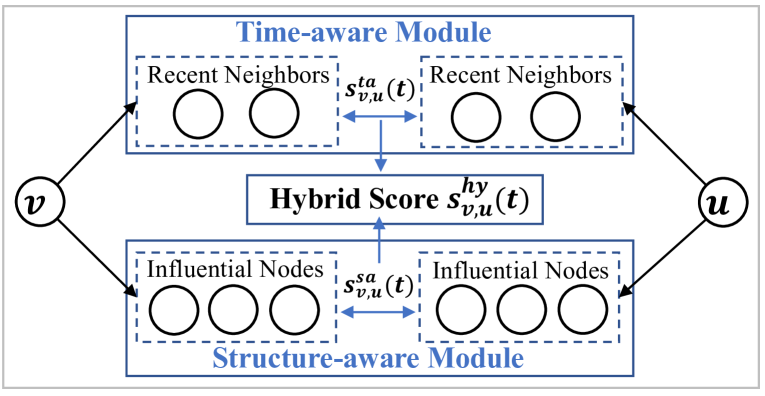
\includegraphics[width=0.6\textwidth]{EAGLE_pic}
    \caption{Архитектура EAGLE: time-aware и structure-aware модули объединяются в гибридную оценку $s_{v,u}^{\text{hy}}(t)$.}
    \label{fig:eagle}
\end{figure}

\subsection{GraphMixer}

Модель GraphMixer (Cong et al., 2023) представляет собой архитектуру для прогнозирования связей в темпоральных графах, разработанную с целью минимизации концептуальной и технической сложности. В отличие от преобладающих подходов, использующих рекуррентные нейронные сети (RNN) или механизмы самовнимания (SAM), GraphMixer построена исключительно на основе многослойных перцептронов (MLP) и операции пулинга соседей, что позволяет достичь конкурентоспособной производительности без усложнения архитектуры. Модель состоит из трёх основных функциональных модулей: кодировщика связей, кодировщика узлов и классификатора связей.

Кодировщик связей обобщает информацию о темпоральных связях каждого узла.
Для узла \(v_i\) берутся \(K\) последних взаимодействий (где \(K\) ---
гиперпараметр, зависящий от датасета), отсортированных по времени. Каждое
взаимодействие в момент \(t\) кодируется конкатенацией вектора признаков связи
\(\mathbf{x}_{ij}^{\text{link}}(t)\) с выходом функции \(\cos(t\boldsymbol{\omega})\)
, которая кодирует timestamp относительного времени \((t_0 - t)\), где \(t_0\) ---
целевой момент прогнозирования. Вектор \(\boldsymbol{\omega} =
\{\alpha^{-(i-1)/\beta}\}_{i=1}^{d}\) содержит фиксированные частотные компоненты,
не обучаемые в процессе тренировки; параметры \(\alpha\) и \(\beta\) подбираются
так, чтобы все временные метки в заданном диапазоне различались. Последовательности
дополняются до длины \(K\) паддингом нулями --- это позволяет модели учитывать
частоту взаимодействий узла. Полученная матрица \(\mathbf{T}_i(t_0)\) размерности
\(K \times d_{\text{input}}\) обрабатывается однослойным MLP-Mixer. Он последовательно
применяет два преобразования: сначала token-mixer обменивается информацией между
взаимодействиями в последовательности, затем channel-mixer обрабатывает признаки
независимо для каждого токена. Оба микшера используют линейные преобразования,
активацию GeLU и LayerNorm. Итоговое представление узла \(v_i\) ---
вектор \(\mathbf{t}_i(t_0)\), получаемый усреднением выходной матрицы channel-mixer.

Кодировщик узлов (node-encoder) предназначен для агрегации статической информации об узле и его ближайшем окружении. Представление узла формируется на основе его собственных признаков \(\mathbf{x}_i^{\text{node}}\) и признаков его \(1\)-соседей, с которыми были зафиксированы взаимодействия за временной интервал \([t_0 - T, t_0]\), где \(T\) — гиперпараметр. Итоговый вектор \(\mathbf{s}_i(t_0)\) вычисляется как сумма собственных признаков узла и среднего значения признаков его соседей: \(\mathbf{s}_i(t_0) = \mathbf{x}_i^{\text{node}} + \text{Mean}\{\mathbf{x}_j^{\text{node}} \mid v_j \in \mathcal{N}(v_i; t_0 - T, t_0)\}\). В случае отсутствия атрибутивных признаков узлов в наборе данных используются one-hot векторы для идентификации узлов.

Классификатор связей (link classifier) является двухслойным MLP, который на основе объединённых представлений пары узлов вычисляет вероятность существования связи между ними в момент времени \(t_0\). Для узлов \(v_i\) и \(v_j\) итоговые представления \(\mathbf{h}_i(t_0) = [\mathbf{s}_i(t_0) \| \mathbf{t}_i(t_0)]\) и \(\mathbf{h}_j(t_0) = [\mathbf{s}_j(t_0) \| \mathbf{t}_j(t_0)]\) конкатенируются и подаются на вход классификатора: \(p_{ij} = \text{MLP}([\mathbf{h}_i(t_0) \| \mathbf{h}_j(t_0)])\).

Важной архитектурной особенностью GraphMixer является рассмотрение темпорального графа как неориентированного. Это позволяет кодировщику узлов извлекать информацию о частоте взаимных связей между узлами в недавнем прошлом, что является значимым признаком для прогнозирования. Выборка ограничивается только \(1\)-соседями с наиболее поздними временными метками, что снижает зашумленность входных данных и уменьшает вычислительную сложность по сравнению с методами, использующими многошаговую или равномерную выборку соседей.

\begin{figure}[ht]
    \centering
    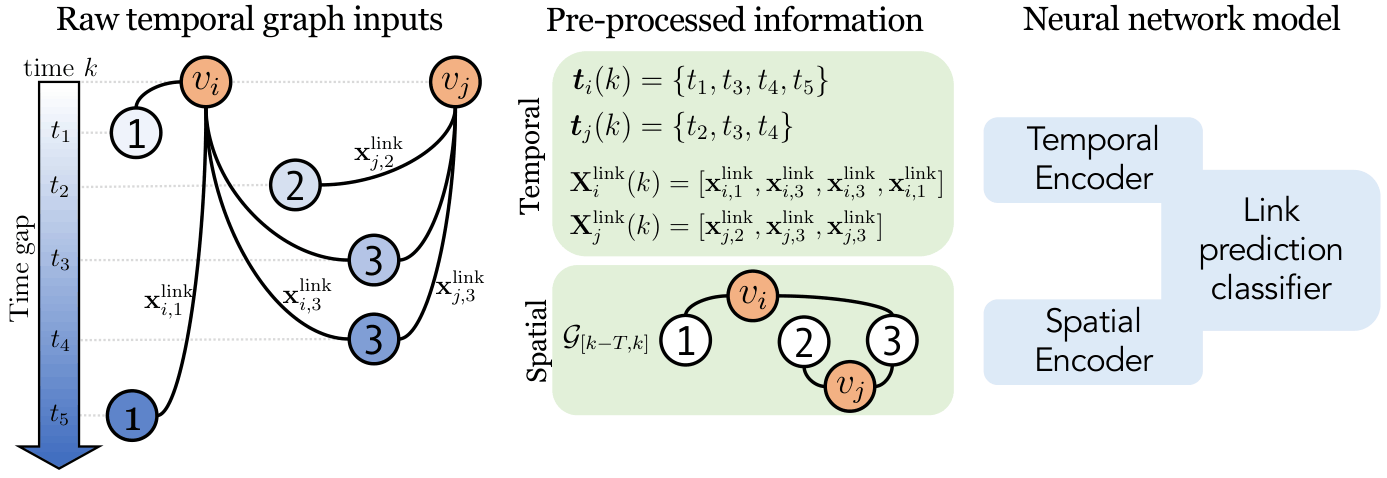
\includegraphics[width=0.85\textwidth]{GraphMixer_pic}
    \caption{Архитектура GraphMixer: темпоральный кодировщик (link-encoder на основе MLP-Mixer) и пространственный кодировщик (node-encoder) подают объединённые представления в классификатор связей.}
    \label{fig:graphmixer}
\end{figure}

\subsection{GLFormer}

Предлагаемая модель GLFormer (Global-Lens Transformer) представляет собой архитектуру для обучения на динамических графах, которая отказывается от классического механизма self-attention в пользу более эффективного адаптивного смешения токенов. Основная идея заключается в том, что успех Transformer-подобных архитектур в значительной степени обусловлен их общей структурой, а не самим механизмом внимания. В связи с этим GLFormer строит процесс обработки последовательностей взаимодействий узлов, комбинируя два ключевых компонента: адаптивный модуль агрегации токенов и иерархический механизм агрегации для расширения временного рецептивного поля.

Пусть для заданного взаимодействия \(e = (u, v, t)\) получены начальные эмбеддинги узлов с помощью некоторой функции внедрения \(f_E\), характерной для существующих методов обучения на темпоральных графах: \(\mathbf{X}_u = f_E(\mathcal{G}_{t-}, u)\). Входными данными для GLFormer служит последовательность эмбеддингов соседей узла \(u\): \(\mathbf{I}_u = [\mathbf{X}_{u_1}, \dots, \mathbf{X}_{u_N}] \in \mathbb{R}^{N \times d}\), где \(N\) — количество рассматриваемых соседей, а \(d\) — размерность эмбеддинга. Основу архитектуры составляют два последовательно применяемых блока: смеситель токенов (token mixer), отвечающий за агрегацию информации между позициями последовательности, и канальный смеситель (channel mixer), моделирующий взаимосвязи между различными признаковыми каналами. Каждый блок дополнен остаточным соединением для стабилизации обучения и интеграции исходных данных.

Адаптивный модуль агрегации токенов выполняет локальное взвешенное суммирование по \(M\) наиболее недавним соседям. Для каждого соседа \(u_i\), взаимодействовавшего в момент \(t_i\), его представление \(H_{i,:}\) считается как взвешенная сумма эмбеддингов предшествующих соседей \(\mathbf{I}_{i-p,:}\), где \(p = 0, \dots, M-1\). Веса агрегации \(\alpha_p^i\) определяются двумя факторами: обучаемыми параметрами \(w_p\), отражающими важность позиционного порядка, и временны\'{м} фактором \(\theta_p^i\), основанным на относительных разностях времён взаимодействий. Итоговый вес задаётся через обучаемый параметр \(\beta\): \(\alpha_p^i = \beta w_p + (1-\beta)\theta_p^i\). Временной фактор вычисляется как softmax от отрицательных временных интервалов: \(\theta_p^i = \frac{\exp(-(t_i - t_{i-p}))}{\sum_{q=0}^{M-1}\exp(-(t_i - t_{i-q}))}\). Так модель адаптирует агрегацию с учётом и порядка взаимодействий, и их временной близости.

Чтобы захватывать долгосрочные зависимости за пределами локального окна, в GLFormer реализован иерархический механизм агрегации: с ростом глубины слоя рецептивное поле расширяется за счёт увеличения шага и числа учитываемых соседей. На слое \(l\) token-mixer использует ядро размера \(K_l\), определяемое множеством смещений \(\mathcal{R}_l = \{p \in \mathbb{Z} \mid s^{l-1} \leq p \leq s^l\}\), где \(s\) --- параметр, контролирующий экспоненциальный рост рецептивного поля. Агрегация на этом уровне: \(\mathbf{H}_{i,:}^{(l)} = \sum_{p \in \mathcal{R}_l} (\alpha_p^{(i)})^{(l)} \mathbf{H}_{\mathrm{TA}, i-p}^{(l-1)}\), где \(\mathbf{H}_{\mathrm{TA}, i-p}^{(l-1)}\) --- выход предыдущего слоя после channel-mixer. Каждый следующий слой работает с более широким временны\'{м} контекстом, что позволяет моделировать и краткосрочную динамику, и долгосрочные закономерности.

Channel-mixer соответствует стандартной реализации из Transformer. После модуля агрегации токенов идут проекция, остаточное соединение и LayerNorm, затем двухслойный feed-forward network с активацией GELU и вторым остаточным соединением. Стек из \(L\) таких слоёв даёт итоговое представление последовательности \(\mathbf{H}_{\mathrm{TA}}^{(L)}\), а финальное темпоральное представление узла \(u\) получается усреднением по всем позициям: \(\mathbf{Z}_u = \frac{1}{N} \sum_{i=1}^N \mathbf{H}_{\mathrm{TA}, i,:}^{(L)}\). По сравнению со стандартным self-attention такая архитектура снижает вычислительную сложность с \(O(N^2)\) до \(O(\sum_{l=1}^L N K_l)\), не теряя при этом способности моделировать сложные временны\'{е} зависимости в динамических графах.

\begin{figure}[ht]
    \centering
    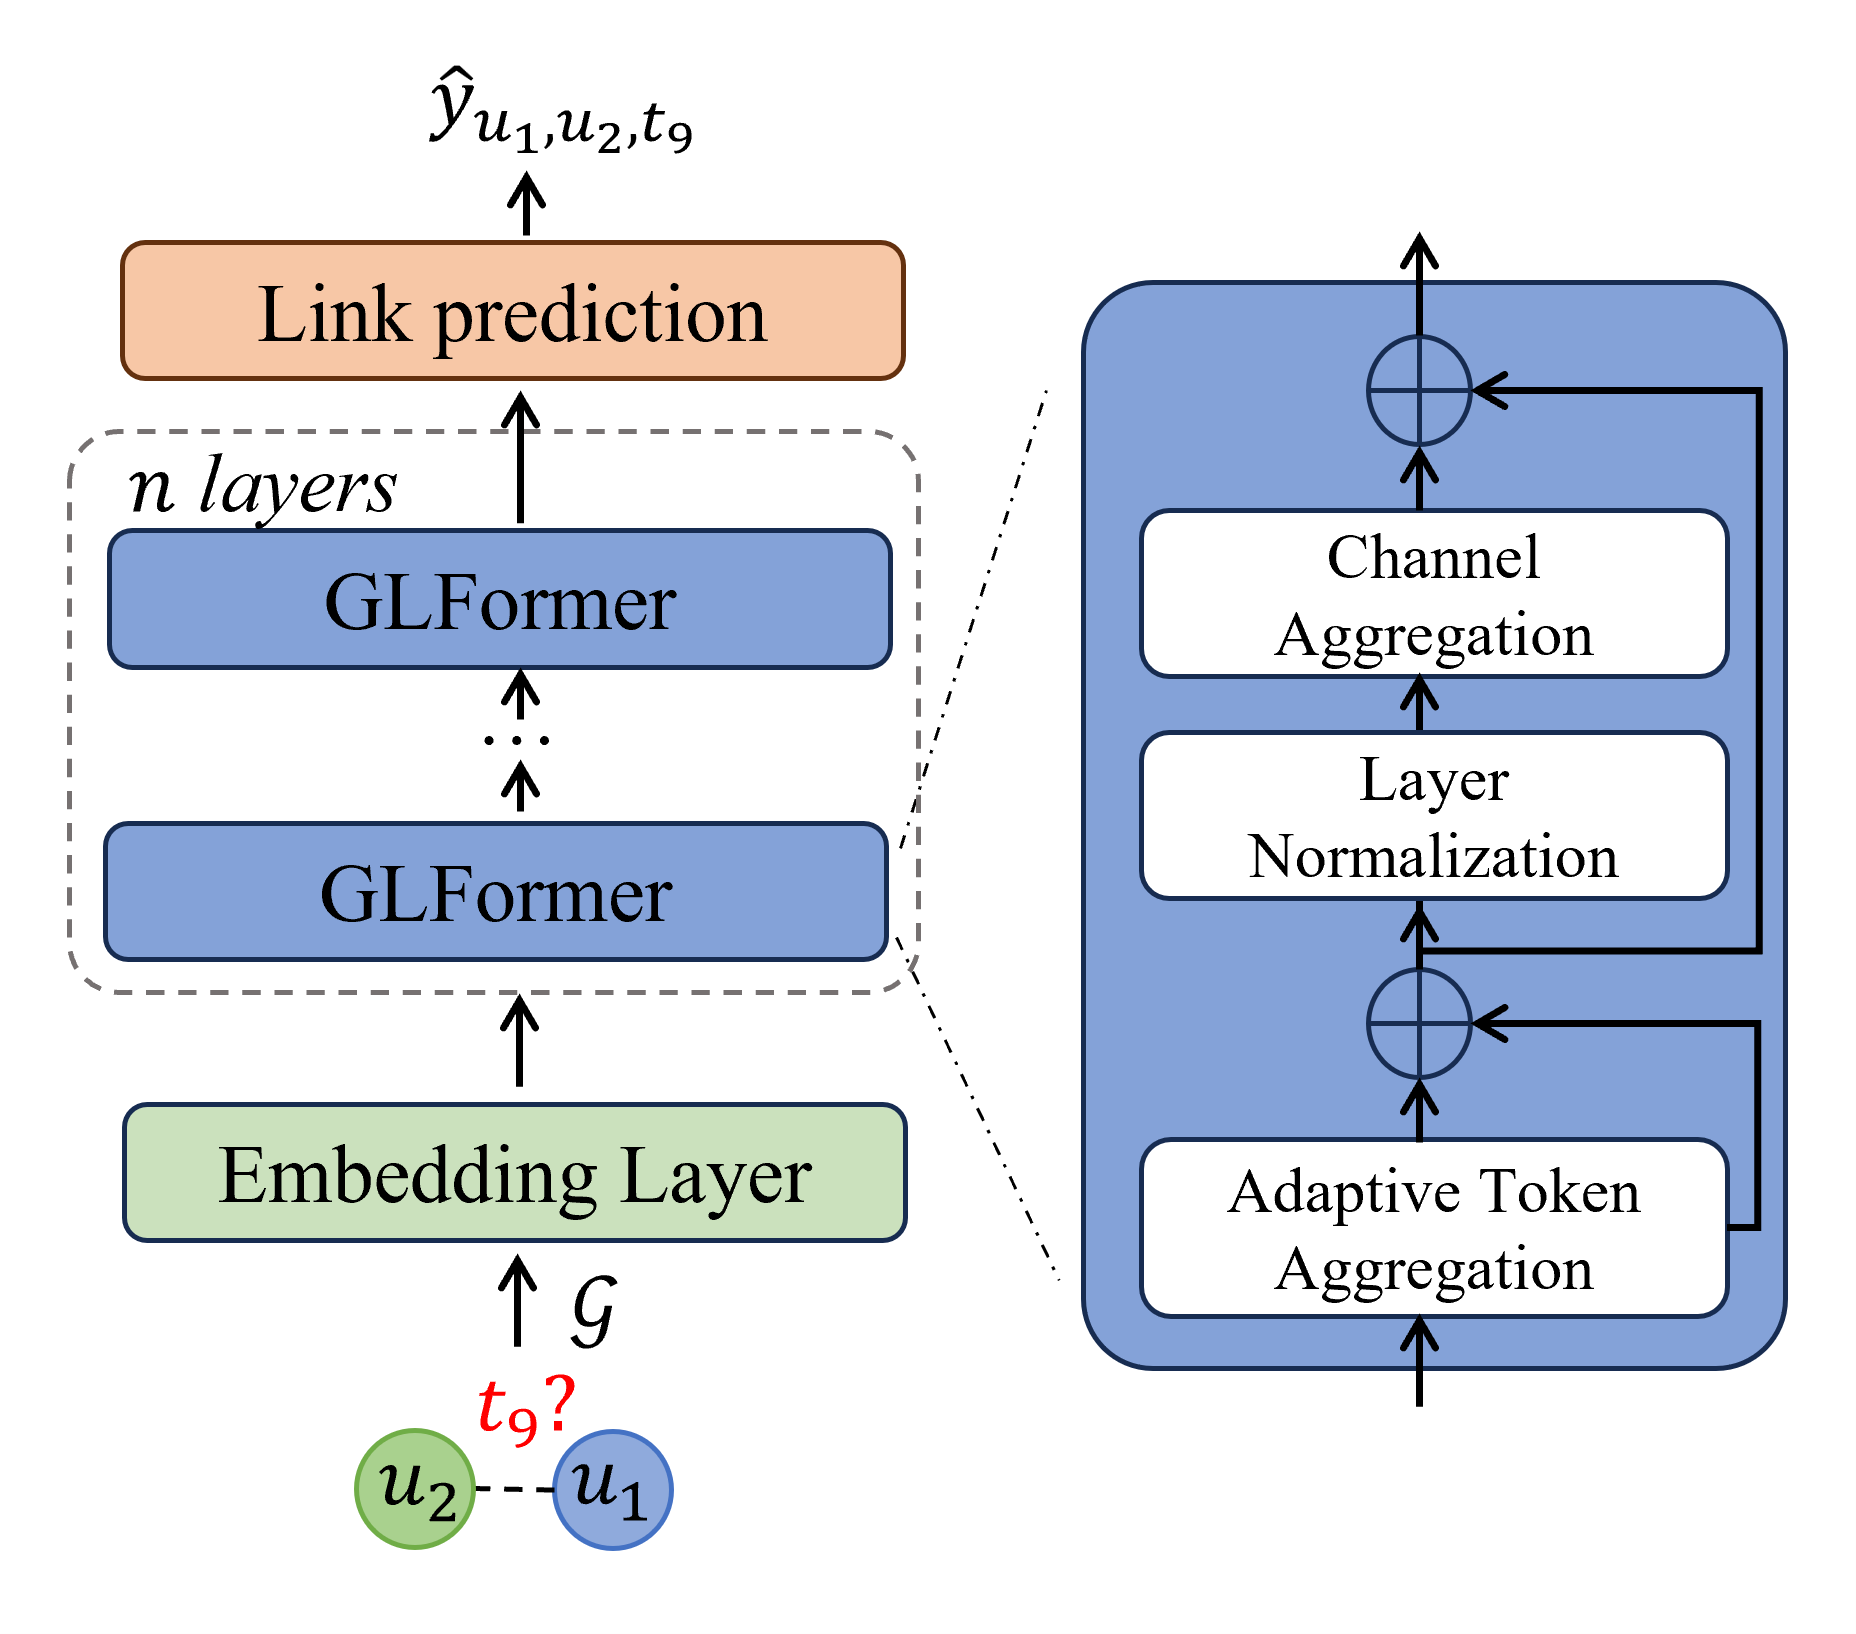
\includegraphics[width=0.5\textwidth]{GLForm_pic}
    \caption{Архитектура GLFormer: стек из $n$ слоёв с адаптивной агрегацией токенов и канальной агрегацией поверх embedding layer; выход подаётся в классификатор предсказания связей.}
    \label{fig:glformer}
\end{figure}

\subsection{DyGFormer}

Предлагаемая архитектура DyGFormer (Dynamic Graph Transformer) основана на применении трансформера для обработки последовательностей исторических взаимодействий узлов. Ключевой принцип заключается в том, чтобы для прогнозирования взаимодействия между узлами-источником \(u\) и узлом-назначением \(v\) в момент времени \(t\) использовать исключительно последовательности их первых соседей (first-hop interactions), предшествующих данному моменту. Такой подход сводит задачу обучения на динамическом графе к задаче анализа последовательностей.

Для каждого узла \(u\) формируется последовательность его исторических взаимодействий \(\mathcal{S}_{u}^{t} = \{(u, u^{\prime}, t^{\prime}) | t^{\prime} < t\} \cup \{(u^{\prime}, u, t^{\prime}) | t^{\prime} < t\}\), аналогично \(\mathcal{S}_{v}^{t}\) для узла \(v\). Из этих последовательностей извлекаются четыре типа признаков: признаки соседей \(\mathbf{X}_{u,N}^{t} \in \mathbb{R}^{|\mathcal{S}_{u}^{t}| \times d_N}\), признаки связей \(\mathbf{X}_{u,E}^{t} \in \mathbb{R}^{|\mathcal{S}_{u}^{t}| \times d_E}\) и кодировка временных интервалов \(\mathbf{X}_{u,T}^{t} \in \mathbb{R}^{|\mathcal{S}_{u}^{t}| \times d_T}\). Кодировка временных интервалов для интервала \(\Delta t' = t - t'\) вычисляется с использованием обучаемых параметров \(w_1, \dots, w_{d_T}\) как \(\left[\cos(w_1 \Delta t'), \sin(w_1 \Delta t'), \dots, \cos(w_{d_T} \Delta t'), \sin(w_{d_T} \Delta t')\right]\).

Ключевое нововведение --- схема кодирования совместной встречаемости соседей (Neighbor Co-occurrence Encoding, NCoE), которая моделирует корреляцию между узлами \(u\) и \(v\). Для каждого соседа в последовательностях \(\mathcal{S}_{u}^{t}\) и \(\mathcal{S}_{v}^{t}\) считается, как часто он встречается в обеих последовательностях сразу --- это даёт двумерный вектор. Собрав такие векторы по всем соседям, получаем признаки совместной встречаемости \(\mathbf{C}_{u}^{t} \in \mathbb{R}^{|\mathcal{S}_{u}^{t}| \times 2}\) и \(\mathbf{C}_{v}^{t} \in \mathbb{R}^{|\mathcal{S}_{v}^{t}| \times 2}\). Затем эти признаки прогоняются через двухслойный перцептрон \(f(\cdot)\) с активацией ReLU: \(\mathbf{X}_{u,C}^{t} = f(\mathbf{C}_{u}^{t}[:, 0]) + f(\mathbf{C}_{u}^{t}[:, 1]) \in \mathbb{R}^{|\mathcal{S}_{u}^{t}| \times d_C}\).

Для работы с длинными историческими последовательностями используется патчинг. Каждая последовательность признаков (например, \(\mathbf{X}_{u,N}^{t}\)) нарезается на непересекающиеся патчи размера \(P\), каждый из которых объединяет \(P\) соседних по времени взаимодействий. Патчи сплющиваются в единые векторы, образуя матрицу \(\mathbf{M}_{u,N}^{t} \in \mathbb{R}^{l_u^t \times (d_N \cdot P)}\), где \(l_u^t = \lceil |\mathcal{S}_{u}^{t}| / P \rceil\) --- число патчей. Размер патча \(P\) растёт вместе с длиной последовательности, так что количество патчей \(l_u^t\) остаётся постоянным и вычислительная сложность не зависит от длины входа.

Далее все типы признаков для узлов \(u\) и \(v\) проецируются в единое пространство размерности \(d\) с помощью обучаемых весов \(\mathbf{W}_*\) и смещений \(\mathbf{b}_*\), после чего конкатенируются: \(\mathbf{Z}_{u}^{t} = [\mathbf{Z}_{u,N}^{t} \| \mathbf{Z}_{u,E}^{t} \| \mathbf{Z}_{u,T}^{t} \| \mathbf{Z}_{u,C}^{t}] \in \mathbb{R}^{l_u^t \times 4d}\) и аналогично \(\mathbf{Z}_{v}^{t} \in \mathbb{R}^{l_v^t \times 4d}\). Полученные представления объединяются в общую входную матрицу \(\mathbf{Z}^{t} = [\mathbf{Z}_{u}^{t}; \mathbf{Z}_{v}^{t}] \in \mathbb{R}^{(l_u^t + l_v^t) \times 4d}\), которая подается на вход кодировщика трансформера.

Кодировщик трансформера состоит из \(L\) слоев, каждый из которых включает блок многоголового самовнимания (Multi-head Self-Attention, MSA) и полносвязную сеть (Feed-Forward Network, FFN). В отличие от оригинальной архитектуры трансформера, в данной работе используется предварительная нормализация слоя (Pre-Layer Normalization) и функция активации GELU. Вычисление для \(l\)-го слоя осуществляется следующим образом:
\[
\begin{aligned}
\mathbf{O}^{t,l} &= \text{MSA}(\text{LN}(\mathbf{Z}^{t,l-1})) + \mathbf{Z}^{t,l-1}, \\
\mathbf{Z}^{t,l} &= \text{FFN}(\text{LN}(\mathbf{O}^{t,l})) + \mathbf{O}^{t,l},
\end{aligned}
\]
где \(\text{MSA}(\cdot)\) — многоголовое самовнимание, \(\text{FFN}(\cdot)\) — полносвязная сеть, \(\text{LN}(\cdot)\) — нормализация слоя, а \(\mathbf{Z}^{t,0} = \mathbf{Z}^{t}\). Выход последнего слоя обозначается как \(\mathbf{H}^{t} = \mathbf{Z}^{t,L} \in \mathbb{R}^{(l_u^t + l_v^t) \times 4d}\).

Финальные временные представления узлов \(u\) и \(v\) получаются путем усреднения соответствующих частей выходной матрицы \(\mathbf{H}^{t}\) с последующим линейным преобразованием:
\[
\begin{aligned}
\mathbf{h}_{u}^{t} &= \text{MEAN}\left(\mathbf{H}^{t} [1 : l_u^t, :]\right) \mathbf{W}_{\text{out}} + \mathbf{b}_{\text{out}}, \\
\mathbf{h}_{v}^{t} &= \text{MEAN}\left(\mathbf{H}^{t} [l_u^t + 1 : l_u^t + l_v^t, :]\right) \mathbf{W}_{\text{out}} + \mathbf{b}_{\text{out}},
\end{aligned}
\]
где \(\mathbf{W}_{\text{out}} \in \mathbb{R}^{4d \times d_{\text{out}}}\) и \(\mathbf{b}_{\text{out}} \in \mathbb{R}^{d_{\text{out}}}\) — обучаемые параметры, \(d_{\text{out}}\) — размерность выходного представления. Полученные векторы \(\mathbf{h}_{u}^{t}\) и \(\mathbf{h}_{v}^{t}\) могут быть использованы для решения задач динамического прогнозирования связей и классификации узлов.

\begin{figure}[ht]
    \centering
    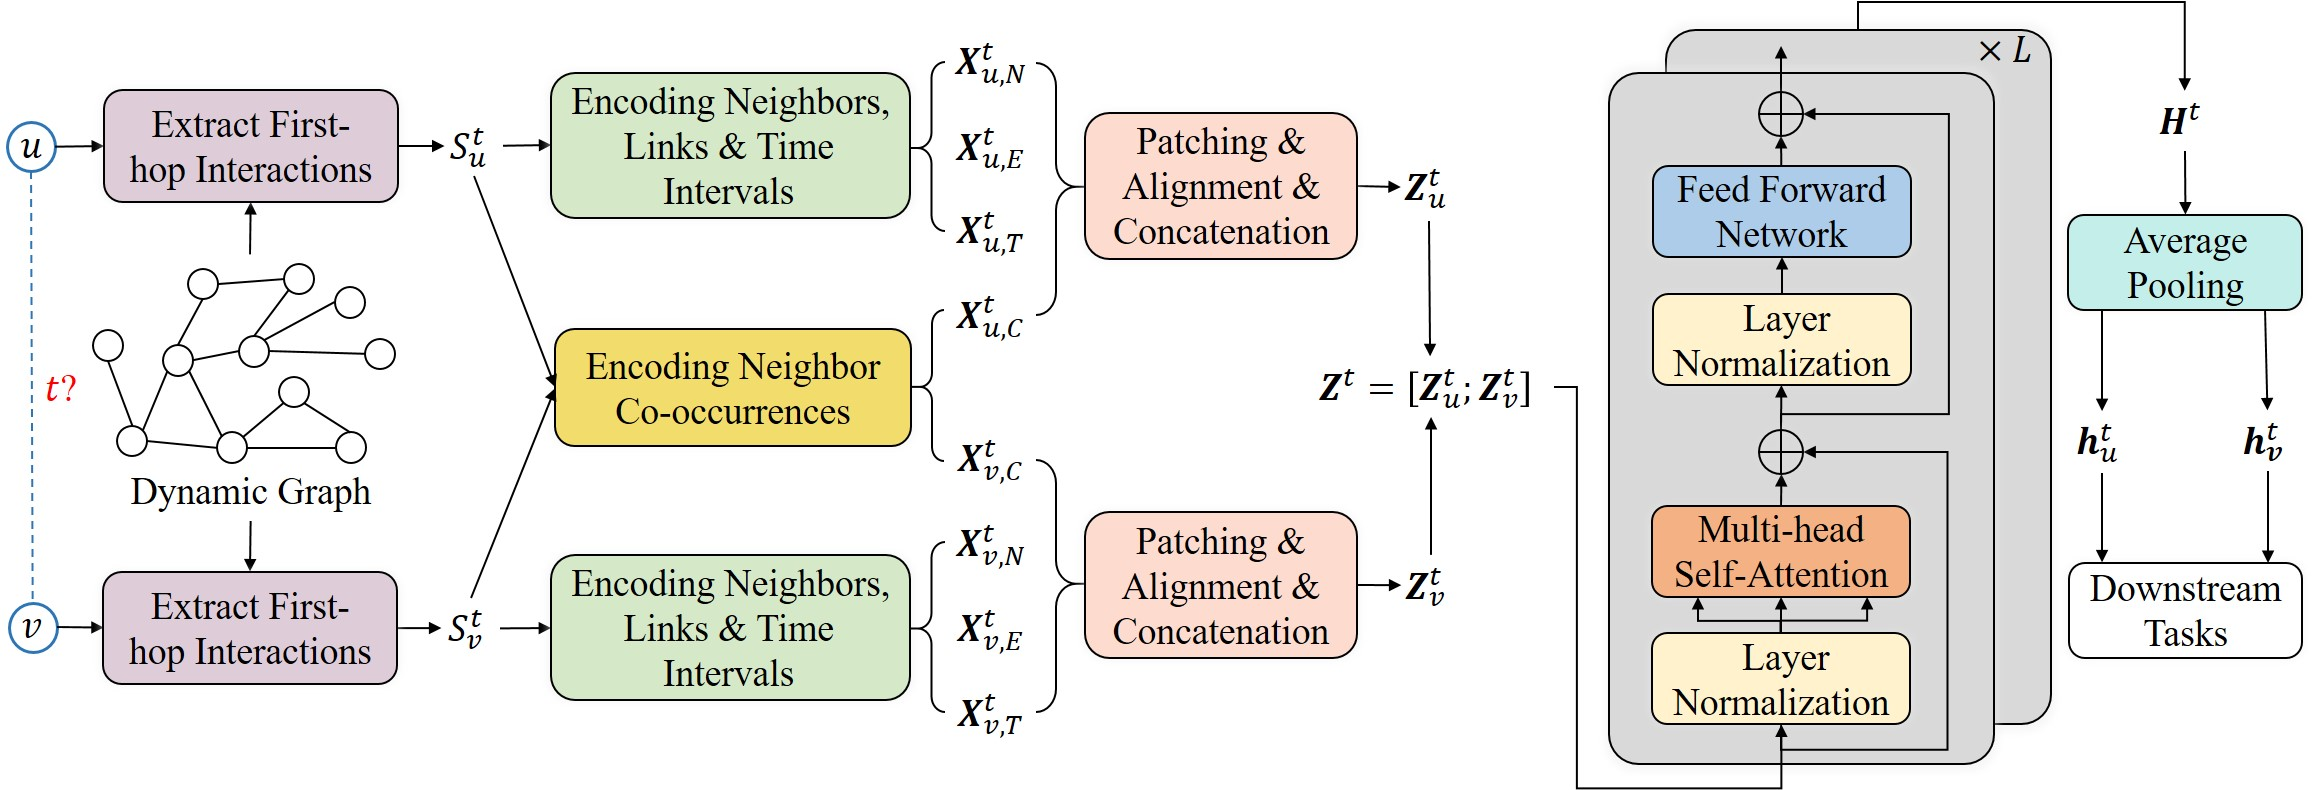
\includegraphics[width=0.95\textwidth]{DyGFormer_pic}
    \caption{Архитектура DyGFormer: патчинг исторических последовательностей взаимодействий узлов \(u\) и \(v\), кодирование совместной встречаемости соседей (NCoE) и обработка трансформером для получения финальных представлений.}
    \label{fig:dygformer}
\end{figure}

\newpage

\section{Эксперименты}

\subsection{Результаты экспериментов}

Все эксперименты проводились на датасете ORBITAAL~--- 10\% рёбер периода 2020-06-01---2020-08-31, что соответствует 6\,143\,581 транзакции между 2\,638\,557 кошельками за 10 дней (подробнее~--- в подразделе «Датасет»). Рёбра разбиты по временному принципу: первые 70\% образуют обучающую выборку, следующие 15\%~--- валидационную, последние 15\%~--- тестовую (подробнее~--- в подразделе «Постановка задачи»). При оценке для каждого положительного ребра сэмплируется один случайный отрицательный кандидат ($N_{\text{neg}} = 1$), то есть модель решает задачу бинарного ранжирования в паре (подробнее~--- в подразделах «Семплирование негативных рёбер» и «Стратегия формирования кандидатов»). Используются метрики MRR, H@1 и H@10, вычисляемые на тестовой выборке (подробнее~--- в подразделе «Метрики качества»). Все эксперименты с нейросетевыми моделями выполнялись на GPU NVIDIA Tesla V100.

\begin{table}[ht]
	\caption{Эксперименты, сравнивающие различные модели}
	\label{table:long_epochs}
	\footnotesize
	\centering
	\begin{tabular}{lrrrr}
		\toprule
		Модель & test MRR & val MRR & test H@1 & test H@10\\
		\midrule
		CN & 0.64 & 0.70 & 0.55 & 0.81\\
		AA & 0.63 & 0.69 & 0.54 & 0.79\\
		CN + MLP & 0.62 & 0.69 & 0.53 & 0.79\\
		Jaccard & 0.55 & 0.63 & 0.45 & 0.75\\
		RF & 0.52 & 0.56 & 0.41 & 0.74\\
		PA & 0.50 & 0.53 & 0.41 & 0.69\\
		Catboost & 0.49 & 0.54 & 0.38 & 0.73\\
		LogReg & 0.35 & 0.36 & 0.26 & 0.52\\
		\bottomrule
		EAGLE & 0.46 & 0.53 & 0.35 & 0.67\\
		DyGFormer & 0.40 & 0.45 & 0.31 & 0.60\\
		GraphMixer & 0.22 & 0.25 & 0.13 & 0.40\\
		GLFormer & 0.09 & 0.07 & 0.11 & 0.20\\
	\end{tabular}
\end{table}

Из таблицы видно, что структурные методы на основе общих соседей (CN, AA) неожиданно превосходят все протестированные нейросетевые модели. Метод CN достигает наилучшего MRR~=~0.64, опережая не только классические ансамблевые методы (RF, CatBoost), но и темпоральные GNN-архитектуры (EAGLE, DyGFormer, GraphMixer, GLFormer). Это указывает на то, что в рассматриваемом датасете транзакционная структура (наличие общих контрагентов) является доминирующим предиктором будущих рёбер, тогда как темпоральные паттерны, которые улавливают GNN, менее информативны. Модель CN~+~MLP с одним признаком (cn\_uu) в данном сравнении показывает результат, близкий к CN и AA, что свидетельствует о том, что MLP способна восстановить структурный сигнал из единственного топологического признака.

\subsection{Аблационное исследование CN + MLP}

Для глубокого понимания поведения модели CN~+~MLP был проведён ряд экспериментов по изменению набора признаков, функции потерь и гиперпараметров обучения. Все эксперименты выполнялись на одном и том же разбиении данных; метрики приводятся по тестовой выборке.

В названиях признаков используются следующие суффиксы: \texttt{\_uu} означает, что величина вычислена на \textit{неориентированном} графе (undirected--undirected); \texttt{\_dir} означает вычисление на \textit{ориентированном} графе (directed).

\begin{table}[ht]
	\caption{Описание экспериментов аблационного исследования CN + MLP}
	\label{table:ablation_desc}
	\footnotesize
	\centering
	\begin{tabular}{lp{0.72\textwidth}}
		\toprule
		ID & Описание \\
		\midrule
		E1      & Минимальный baseline: PairMLP обучается только на одном структурном признаке~cn\_uu. \\
		E2      & К baseline добавлены два близких топологических признака: log1p\_cn\_uu и aa\_uu. \\
		E3      & Полный набор из 7 признаков (включая directed-варианты и degree-based признаки); функция потерь~--- BPR. \\
		E4      & Повтор E3 с тем же набором из 7 признаков, но с заменой BPR на BCE loss. \\
		E5      & Один признак cn\_uu с cosine learning-rate scheduler и явно отключёнными node features. \\
		E6\_lr4 & Тот же одно-признаковый вариант (cn\_uu), но с уменьшенным learning rate и укороченным графиком обучения. \\
		E7\_e2  & Набор из E2 (cn\_uu + log1p\_cn\_uu + aa\_uu) с укороченным обучением и ранней остановкой. \\
		E8\_all & Полный набор из 7 признаков без dropout, с уменьшенным learning rate и коротким training schedule. \\
		E9\_big & Один признак cn\_uu, но с более широкой и глубокой MLP: проверяется, ограничивает ли ёмкость модели результат. \\
		\bottomrule
	\end{tabular}
\end{table}

\begin{table}[ht]
	\caption{Аблационное исследование: набор признаков и гиперпараметры CN + MLP}
	\label{table:ablation_cnmlp}
	\footnotesize
	\centering
	\begin{tabular}{llrrr}
		\toprule
		ID & Признаки / условие & MRR & H@1 & H@10 \\
		\midrule
		E6\_lr4 & cn\_uu, сниженный LR                      & \textbf{0.6164} & \textbf{0.5326} & \textbf{0.7881} \\
		E5      & cn\_uu, cosine scheduler                  & 0.6061 & 0.5249 & 0.7721 \\
		E1      & cn\_uu (baseline)                         & 0.6026 & 0.5220 & 0.7669 \\
		E9\_big & cn\_uu, увеличенная MLP                   & 0.5965 & 0.5176 & 0.7576 \\
		E7\_e2  & cn\_uu + log1p\_cn\_uu + aa\_uu, короткое обучение & 0.5775 & 0.4914 & 0.7480 \\
		E2      & cn\_uu + log1p\_cn\_uu + aa\_uu           & 0.5721 & 0.4871 & 0.7407 \\
		E8\_all & 7 признаков, короткое обучение, без dropout & 0.3300 & 0.2479 & 0.4783 \\
		E4      & 7 признаков, BCE loss                     & 0.3261 & 0.2544 & 0.4559 \\
		E3      & 7 признаков, BPR loss                     & 0.3075 & 0.2301 & 0.4431 \\
		\bottomrule
	\end{tabular}
\end{table}

По результатам аблационного исследования можно сформулировать следующие выводы.

\paragraph{Единственный признак cn\_uu является наиболее информативным.}
Базовый эксперимент E1 с одним признаком (cn\_uu) демонстрирует MRR~=~0.603, тогда как добавление близких топологических признаков log1p\_cn\_uu и aa\_uu (E2) снижает MRR до~0.572. Это означает, что дополнительные признаки вносят избыточность или шум, а не дополнительный сигнал: log1p\_cn\_uu является монотонным преобразованием cn\_uu, а aa\_uu сильно с ним коррелирует.

\paragraph{Расширение набора до 7 признаков резко ухудшает качество.}
Эксперименты E3, E4 и E8\_all используют полный набор из семи признаков (directed-варианты, Jaccard, preferential attachment) и дают MRR в диапазоне 0.31--0.33 --- примерно вдвое хуже однопризнакового базового варианта. Причина простая: менее релевантные признаки глушат полезный сигнал cn\_uu. Замена BPR-loss на BCE (E3 vs.\ E4) картину не меняет --- оба варианта заметно проигрывают единственному признаку.

\paragraph{Размер MLP не влияет на качество при единственном признаке.}
Эксперимент E9\_big с расширенной архитектурой MLP на том же единственном признаке cn\_uu даёт MRR~=~0.597 --- чуть хуже базового E1~(0.603). Узкое место здесь не ёмкость модели, а сам вход: один скалярный признак просто не даёт модели больше информации, сколько слоёв ни добавляй.

\paragraph{Тюнинг гиперпараметров обучения улучшает базовый результат.}
Лучший тестовый MRR получен в E6\_lr4~(0.616) --- тот же единственный признак cn\_uu, но с уменьшенным learning rate и более коротким расписанием обучения. Добавление cosine scheduler в E5 тоже даёт небольшой прирост относительно базового E1. Вывод: при фиксированном наборе признаков аккуратный тюнинг режима обучения работает лучше, чем добавление новых признаков.

\paragraph{Общий вывод.}
В рассматриваемой задаче признак Common Neighbors (cn\_uu) является единственным значимым топологическим дескриптором для MLP-модели. Расширение признакового пространства не только не помогает, но стабильно ухудшает результат. Оптимальная конфигурация CN~+~MLP сводится к минимальному набору признаков с тщательно подобранным learning rate.

\newpage

\section{Библиотека}

\subsection{Назначение и значимость}

  В рамках проекта была разработана библиотека \texttt{payment-graph-forecasting}, предназначенная для обучения, оценки и анализа моделей на темпоральных графах
  платежей. Необходимость создания именно библиотеки, а не набора отдельных исследовательских скриптов, связана с несколькими причинами. Во-первых, для задач на
  темпоральных графах требуется единый способ описания эксперимента, работы с данными, запуска моделей и оценки результатов. Во-вторых, в практической работе важно
  не только воспроизвести отдельную модель, но и иметь возможность расширять систему новыми моделями, источниками данных и вычислительными backend'ами без
  переписывания всего экспериментального контура. В-третьих, для прикладного использования принципиальны воспроизводимость, тестируемость и наличие поддерживаемой
  документации.

  Таким образом, предлагаемая система решает не только исследовательскую задачу сравнения моделей на темпоральных графах, но и инженерную задачу построения целостной
  программной платформы для работы с такими моделями. В отличие от benchmark-oriented решений, ориентированных прежде всего на оффлайн-эксперименты на заранее
  подготовленных датасетах, библиотека \texttt{payment-graph-forecasting} проектировалась как расширяемая библиотечная поверхность с единым API, типизированной
  конфигурацией, примерами запуска, документацией и автоматическими тестами.

  \subsection{Формальная архитектура}

  Канонической пользовательской поверхностью в репозитории является пакет \path{payment_graph_forecasting.*}, тогда как директория \path{src/*} сохранена главным
  образом как слой legacy-реализаций и внутренней исследовательской логики. Такое разделение позволяет, с одной стороны, сохранить уже реализованные модели и
  экспериментальные сценарии, а с другой стороны, предоставить поверх них единый библиотечный интерфейс.

  Архитектурно библиотека состоит из 11 основных пакетных областей:
  \begin{center}
  \begin{tabular}{ll}
  \texttt{config} & типизированные конфигурации и загрузка YAML-спецификаций \\
  \texttt{models} & адаптеры моделей и реестр поддерживаемых архитектур \\
  \texttt{training} & процедуры обучения и runtime-обёртки \\
  \texttt{evaluation} & единый слой оценки качества и ranking loop \\
  \texttt{data} & доступ к данным в формате \texttt{stream\_graph} \\
  \texttt{analysis} & анализ и описание темпорального графа \\
  \texttt{sampling} & стратегии негативного семплирования и temporal sampling \\
  \texttt{cuda} & проверка доступности ускоренных backend'ов \\
  \texttt{graph\_metrics} & графовые примитивы времени выполнения \\
  \texttt{experiments} & единый launcher, runner'ы и HPO entrypoints \\
  \texttt{infra} & доступ к данным, runtime-инфраструктура и optional extensions \\
  \end{tabular}
  \end{center}

  На уровне репозитория структура проекта может быть кратко представлена следующим образом:
  \begin{center}
  \begin{tabular}{ll}
  \texttt{payment-graph-forecasting/} & корневая директория проекта \\
  \texttt{\ \ payment\_graph\_forecasting/} & канонический библиотечный API \\
  \texttt{\ \ exps/examples/} & примеры YAML-конфигураций \\
  \texttt{\ \ docs/} & пользовательская документация \\
  \texttt{\ \ tests/} & автоматические тесты \\
  \texttt{\ \ src/} & legacy/internal реализации и backend-код \\
  \end{tabular}
  \end{center}

  Формально описание эксперимента задаётся типизированным объектом \texttt{ExperimentSpec}. Он состоит из нескольких dataclass-компонент:
  \begin{itemize}
      \item \texttt{ExperimentMetadata} --- имя эксперимента, модель и служебные теги;
      \item \texttt{DataConfig} --- источник данных, пути к файлам, доля периода, параметры разбиения и кэширования;
      \item \texttt{SamplingConfig} --- стратегия негативного семплирования, число соседей и выбор backend'а;
      \item \texttt{TrainingConfig} --- число эпох, размер батча, скорость обучения и другие параметры обучения;
      \item \texttt{RuntimeConfig} --- устройство выполнения, mixed precision, \texttt{dry\_run}, директория вывода;
      \item \texttt{UploadConfig} --- параметры выгрузки артефактов;
      \item \texttt{model} --- словарь модельно-специфичных параметров.
  \end{itemize}

  После загрузки YAML-спецификации библиотека преобразует её в \texttt{ExperimentSpec}, а затем передаёт в слой адаптеров моделей. Базовый контракт этого слоя задают
  классы \texttt{BaseModelAdapter} и \texttt{BaseRunnerAdapter}. На уровне интерфейсов они опираются на два основных объекта:
  \begin{itemize}
      \item \texttt{ModelExecutionPlan} --- канонический план запуска модели;
      \item \texttt{LaunchResult} --- унифицированный результат выполнения.
  \end{itemize}
  Такое разделение позволяет отделить библиотечный API от конкретных runner'ов и при этом сохранить совместимость с уже существующими реализациями в \path{src/*}.

  Для краткой формализации объёма и структуры библиотеки приведём её основные количественные характеристики (таблица~\ref{tab:library_characteristics}).

  \begin{table}[h]
  \centering
  \caption{Формальные характеристики библиотеки \texttt{payment-graph-forecasting}}
  \label{tab:library_characteristics}
  \begin{tabular}{l r}
  \toprule
  Характеристика & Значение \\
  \midrule
  Основных пакетных областей канонического API & 11 \\
  Поддерживаемых моделей в реестре & 7 \\
  Reference YAML-конфигураций в \path{exps/examples/} & 7 \\
  Поддерживаемых источников данных типа \texttt{stream\_graph} & 6 \\
  Backend'ов для runtime-примитивов & 3 \\
  Тестовых файлов в каталоге \path{tests/} & 47 \\
  \bottomrule
  \end{tabular}
  \end{table}

  \subsection{Поддерживаемые модели и данные}

  На уровне моделей библиотека предоставляет единый интерфейс для семи семейств методов:
  \begin{itemize}
      \item \texttt{graphmixer};
      \item \texttt{sg\_graphmixer};
      \item \texttt{eagle};
      \item \texttt{glformer};
      \item \texttt{hyperevent};
      \item \texttt{pairwise\_mlp};
      \item \texttt{dygformer}.
  \end{itemize}

  Важно, что библиотечный API не сводится к простому переэкспорту кода моделей. Между пользовательской конфигурацией и конкретной реализацией введён слой адаптеров,
  который приводит параметры эксперимента к унифицированному виду, формирует стандартные runtime-аргументы и связывает верхнеуровневый вызов с конкретным runner'ом.
  За счёт этого добавление новой модели означает не только реализацию самой архитектуры, но и её включение в общую схему запуска, обучения и оценки.

  Единицей работы с данными в библиотеке является \texttt{stream graph}, хранимый в parquet-формате. Канонический слой \texttt{payment\_graph\_forecasting.data}
  задаёт классы \texttt{StreamGraphDataset}, \texttt{StreamGraphSelection} и \texttt{StreamGraphDescriptor}, а также функцию \texttt{open\_stream\_graph}. Библиотека
  поддерживает полный граф, хронологический префикс периода и выбор диапазона дат. Обязательный набор колонок канонического представления включает \texttt{src\_idx},
  \texttt{dst\_idx}, \texttt{timestamp}, \texttt{btc} и \texttt{usd}. Кроме того, слой \texttt{infra.datasets} поддерживает шесть типов источников данных:
  \texttt{stream\_graph}, \texttt{orbitaal\_stream\_graph}, \texttt{jodie\_csv}, \texttt{jodie\_wikipedia}, \texttt{edge\_table\_csv} и
  \texttt{edge\_table\_parquet}. Тем самым библиотека решает не только задачу запуска моделей, но и задачу приведения разнородных источников к единому внутреннему
  формату.

  \subsection{Система с точки зрения пользователя}

  С практической точки зрения библиотека поддерживает три пользовательских сценария.

  Первый сценарий --- декларативный запуск экспериментов через YAML-конфигурации. Пользователь описывает эксперимент в виде спецификации, после чего библиотека
  загружает её, строит \texttt{ExperimentSpec}, выбирает нужный адаптер и запускает соответствующий runner. В репозитории присутствуют готовые reference-конфигурации
  для всех поддерживаемых моделей в директории \path{exps/examples/}.

  Второй сценарий --- прямое использование библиотечного API из Python-кода. На верхнем уровне пакет экспортирует, в частности, следующие объекты:
  \begin{itemize}
      \item \texttt{load\_experiment\_spec};
      \item \texttt{build\_execution\_plan};
      \item \texttt{launch\_experiment};
      \item \texttt{open\_stream\_graph};
      \item \texttt{analyze\_stream\_graph};
      \item \texttt{TemporalGraphSampler};
      \item \texttt{CommonNeighbors};
      \item \texttt{describe\_cuda\_capabilities}.
  \end{itemize}

  Третий сценарий --- взаимодействие с ИИ-ассистентом, ориентированным на библиотечный способ работы с системой. В документации вынесен отдельный prompt, в рамках
  которого агент может сопровождать пользователя при установке окружения, подготовке данных, выборе модели, запуске эксперимента, отладке и расширении библиотеки.
  Таким образом, у системы есть не только программный и конфигурационный интерфейс, но и дополнительный сценарий пользовательского сопровождения.

  Пример YAML-спецификации эксперимента может быть представлен следующим образом:
  \begin{lstlisting}[basicstyle=\ttfamily\small,frame=single]
  experiment:
    name: eagle_library_smoke
    model: eagle

  data:
    source: stream_graph
    parquet_path: /tmp/sg_baselines_data/stream_graph.parquet
    features_path: /tmp/sg_baselines_data/features_10.parquet
    fraction: 0.10

  sampling:
    strategy: tgb_mixed
    num_neighbors: 20
    n_random_neg: 50
    n_hist_neg: 50
    backend: auto

  training:
    epochs: 5
    batch_size: 200
    lr: 0.001

  runtime:
    device: auto
    output_dir: /tmp/eagle_results

  model:
    edge_feat_dim: 2
    node_feat_dim: 15
  \end{lstlisting}

  Соответствующий запуск может быть выполнен следующей командой:
  \begin{lstlisting}[basicstyle=\ttfamily\small,frame=single]
  ./venv/bin/python -m payment_graph_forecasting.experiments.launcher \
    --config exps/examples/eagle_library.yaml
  \end{lstlisting}

  \subsection{Обоснование выбранных решений}

  Выбранная архитектура библиотеки является оптимальной в том смысле, что она разделяет изменяющиеся и стабильные части системы. Типизированная конфигурация делает
  запуск экспериментов формализованным и воспроизводимым. Слой адаптеров моделей позволяет подключать новые архитектуры без изменения пользовательского API. Единый
  формат \texttt{stream graph} снимает необходимость подстраивать конвейер обучения под каждую модель отдельно. Выделение вычислительно затратных операций в
  отдельные runtime-примитивы позволяет независимо оптимизировать их реализацию, не меняя внешний интерфейс библиотеки.

  Эта идея особенно важна для операций, связанных с темпоральным семплированием соседей и вычислением графовых метрик. Для них в библиотеке предусмотрены
  альтернативные backend'ы на Python, C++ и CUDA. Тем самым одна и та же библиотечная поверхность может использовать как базовую интерпретируемую реализацию, так и
  ускоренные варианты для более тяжёлых сценариев. Подробный экспериментальный анализ этих решений и сравнение времени работы будет приведён в следующем разделе,
  посвящённом CUDA-модулю.

  С точки зрения связи с известными аналогами такой подход позволяет рассматривать библиотеку не только как средство воспроизведения отдельных моделей, но и как
  более общий программный слой для постановки и запуска экспериментов. По сравнению с решениями, ориентированными прежде всего на оффлайн-бенчмарки, в
  \texttt{payment-graph-forecasting} больший акцент сделан на типизированной конфигурации, библиотечном API, расширяемости, тестировании и документированном
  пользовательском сценарии.

  \subsection{Документация, тестирование и демонстрация}

  Важной характеристикой библиотеки является готовность к демонстрации и сопровождению. В репозитории присутствуют:
  \begin{itemize}
      \item основной \texttt{README.md} с описанием канонической поверхности библиотеки;
      \item отдельная документация в \path{docs/}, включая описание CUDA-модуля, evaluation protocol'ов и сценариев работы;
      \item примеры YAML-конфигураций в \path{exps/examples/};
      \item единый launcher и вспомогательные CLI-команды;
      \item автоматические тесты в \path{tests/}.
  \end{itemize}

  Тестовое покрытие библиотеки является достаточно широким: в каталоге \path{tests/} содержится 47 тестовых файлов. Они проверяют, в частности, библиотечный API,
  слой конфигураций, launcher, модельные runner'ы, работу с \texttt{stream\_graph}, доступ к данным, negative sampling, temporal sampling, graph metrics, training/
  evaluation API, совместимость с legacy-слоем и инфраструктурные компоненты. Тем самым библиотека сопровождается не только документацией, но и формализованным
  набором проверок корректности.

  С точки зрения демонстрации система может быть показана в работе несколькими способами: через запуск YAML-спецификации, через прямой вызов Python API, через анализ
  графа с помощью вспомогательных скриптов и через использование ИИ-ассистента. Это означает, что библиотека удовлетворяет требованию демонстрируемости как
  программный проект и одновременно обладает поддерживаемой пользовательской документацией.

  В совокупности это позволяет рассматривать \texttt{payment-graph-forecasting} не как набор разрозненных исследовательских скриптов, а как целостную библиотеку для
  работы с темпоральными графами платежей, имеющую формализованную архитектуру, единый пользовательский интерфейс, воспроизводимый сценарий запуска, поддержку
  документации и развитое тестовое покрытие.

\section{CUDA}

Одной из ключевых инженерных задач в рамках проекта стало ускорение вычислительно затратных операций, возникающих при обучении моделей на темпоральных графах. Для
  этого в библиотеке был реализован отдельный CUDA-модуль, предоставляющий GPU-ускоренные примитивы для работы с графом и при этом встроенный в общий API библиотеки,
  а не оформленный как внешняя утилита. В текущей реализации модуль охватывает два базовых алгоритма: поиск последних по времени соседей узла и вычисление числа
  общих соседей для пары узлов. Для каждого из этих примитивов предусмотрены три backend'а: \texttt{python}, \texttt{cpp} и \texttt{cuda}. Выбор backend'а может
  осуществляться явно или автоматически, а для обучения моделей он задаётся через конфигурационный параметр \texttt{sampling.backend}.

  С точки зрения пользовательского интерфейса CUDA-часть библиотеки не образует отдельного способа запуска, а включается в общий библиотечный сценарий. На уровне
  Python API в библиотеку вынесены следующие объекты:
  \begin{itemize}
      \item \texttt{TemporalGraphSampler};
      \item \texttt{CommonNeighbors};
      \item \texttt{describe\_cuda\_capabilities}.
  \end{itemize}
  На уровне конфигурации эксперимента подключение ускоренного пути для моделей, использующих темпоральное семплирование, выполняется через YAML-спецификацию
  следующего вида:
  \begin{lstlisting}[basicstyle=\ttfamily\small,frame=single]
  sampling:
    backend: cuda
  \end{lstlisting}
  В частности, для DyGFormer этот параметр действительно маршрутизирует обучение в CUDA-реализацию подготовки батчей, использующую \texttt{TemporalGraphSampler}
  внутри стандартного библиотечного запуска.

  \subsection{Поиск временных соседей}

  Первым реализованным примитивом является поиск последних по времени соседей узла. Для узла $u$ и момента времени $t$ требуется найти не более $K$ последних
  исходящих рёбер $(u, v, \tau)$, удовлетворяющих условию $\tau < t$. Именно эта операция лежит в основе подготовки входных данных для моделей семейства GraphMixer,
  GLFormer и DyGFormer. В библиотеке граф хранится в CSR-подобной структуре, где рёбра отсортированы по источнику, а внутри каждой строки --- по возрастанию времени.
  Тогда для каждого запроса $(u,t)$ сначала определяется правая граница среди рёбер узла $u$ по условию \texttt{timestamp < t}, после чего выбираются последние $K$
  элементов слева от этой границы.

  В \texttt{python}-backend эта логика реализована через NumPy-массивы и последовательный проход по батчу запросов. В \texttt{cpp}-backend используется та же
  структура данных, но критические участки вынесены в C++-расширение. В \texttt{cuda}-backend CSR-структура переносится в память GPU один раз, а дальнейшие операции
  поиска соседей и извлечения признаков выполняются уже на устройстве. Помимо собственно поиска соседей, примитив поддерживает отдельную стадию \texttt{featurize},
  которая собирает признаки узлов соседей, признаки рёбер и относительные временные интервалы.

  Для оценки эффективности данного примитива был проведён набор бенчмарков на синтетических данных, в которых варьировались размер батча, число соседей $K$ и размер
  искусственно сгенерированного графа. Подчеркнём, что в данном подразделе речь идёт именно о синтетических данных, а не о полном обучении модели на реальном
  датасете. Результаты приведены в таблице~\ref{tab:cuda_sampling_bench}.

  \begin{table}[h]
  \centering
  \caption{Бенчмарк поиска временных соседей и извлечения признаков на синтетических данных}
  \label{tab:cuda_sampling_bench}
  \begin{tabular}{l l r r r r}
  \toprule
  Сценарий & Backend & Sample, ms & Feat, ms & Total, ms & Ускорение \\
  \midrule
  graphmixer\_small & python & 2.74 & 4.82 & 7.55 & 1.0x \\
  graphmixer\_small & cpp    & 0.07 & 0.14 & 0.21 & 35.9x \\
  graphmixer\_small & cuda   & 0.08 & 0.07 & 0.15 & 49.9x \\
  \midrule
  dygformer\_small  & python & 3.04 & 8.46 & 11.49 & 1.0x \\
  dygformer\_small  & cpp    & 0.40 & 3.63 & 4.04 & 2.8x \\
  dygformer\_small  & cuda   & 0.09 & 0.09 & 0.18 & 64.2x \\
  \midrule
  dygformer\_medium & python & 14.10 & 48.30 & 62.33 & 1.0x \\
  dygformer\_medium & cpp    & 2.12 & 32.07 & 34.22 & 1.8x \\
  dygformer\_medium & cuda   & 0.12 & 0.22 & 0.34 & 183.7x \\
  \midrule
  dygformer\_large  & python & 14.20 & 49.16 & 63.53 & 1.0x \\
  dygformer\_large  & cpp    & 2.14 & 33.08 & 35.26 & 1.8x \\
  dygformer\_large  & cuda   & 0.13 & 0.23 & 0.36 & 175.9x \\
  \midrule
  real\_scale       & python & 2.79 & 5.89 & 8.64 & 1.0x \\
  real\_scale       & cpp    & 0.38 & 2.21 & 2.61 & 3.3x \\
  real\_scale       & cuda   & 0.09 & 0.09 & 0.18 & 48.5x \\
  \bottomrule
  \end{tabular}
  \end{table}

  Полученные результаты показывают, что ускорение особенно велико в сценариях, характерных для DyGFormer, где число соседей $K$ велико. В наиболее показательном
  случае \texttt{dygformer\_medium} CUDA-реализация уменьшает суммарное время операций \texttt{sample + featurize} с $62.33$~мс до $0.34$~мс, что соответствует
  ускорению в $183.7$ раза относительно \texttt{python}-backend. Тем самым CUDA-путь делает подготовку темпорального контекста существенно менее затратной даже при
  больших значениях $K$ и размере батча.

  \subsection{Common Neighbors}

  Вторым реализованным примитивом является точное вычисление числа общих соседей для пары узлов:
  \[
  CN(u,v)=|N(u)\cap N(v)|.
  \]
  Этот признак широко используется как сильная эвристика в задачах link prediction и может быть полезен как самостоятельно, так и в составе более сложных моделей.

  В библиотеке реализованы три backend'а для данной операции. В \texttt{python}-backend используется работа с CSR-представлением через \texttt{scipy}. В
  \texttt{cpp}-backend применяется классический алгоритм sorted merge двух отсортированных списков соседей, имеющий сложность $O(d_u+d_v)$ для пары узлов степени
  $d_u$ и $d_v$. В \texttt{cuda}-backend реализован другой подход: множество соседей узла упаковывается в битовое представление, после чего число общих соседей
  вычисляется как сумма значений \texttt{popcount} для побитового пересечения двух bitset'ов. Таким образом, утверждение о реализации через bitset действительно
  соответствует коду.

  Как и в предыдущем подразделе, бенчмарки для \texttt{CommonNeighbors} проводились на синтетически сгенерированных графах различной плотности. Это важно, поскольку
  именно плотность графа определяет, какой backend оказывается наиболее выгодным. Результаты приведены в таблице~\ref{tab:cuda_cn_bench}.

  \begin{table}[h]
  \centering
  \caption{Бенчмарк вычисления Common Neighbors на синтетических данных}
  \label{tab:cuda_cn_bench}
  \begin{tabular}{l l r r r}
  \toprule
  Сценарий & Backend & Median, ms & p95, ms & Ускорение \\
  \midrule
  sparse\_like\_bitcoin & python & 0.42 & 0.48 & 1.0x \\
  sparse\_like\_bitcoin & cpp    & 0.07 & 0.08 & 5.9x \\
  sparse\_like\_bitcoin & cuda   & 1.18 & 1.24 & 0.4x \\
  \midrule
  breakeven             & python & 1.27 & 1.36 & 1.0x \\
  breakeven             & cpp    & 0.57 & 0.62 & 2.2x \\
  breakeven             & cuda   & 0.73 & 0.81 & 1.7x \\
  \midrule
  dense\_small          & python & 2.00 & 2.08 & 1.0x \\
  dense\_small          & cpp    & 1.02 & 1.06 & 1.9x \\
  dense\_small          & cuda   & 0.42 & 0.48 & 4.8x \\
  \midrule
  dense\_medium         & python & 8.51 & 8.88 & 1.0x \\
  dense\_medium         & cpp    & 5.05 & 5.21 & 1.7x \\
  dense\_medium         & cuda   & 0.71 & 0.75 & 12.0x \\
  \midrule
  dense\_large          & python & 35.79 & 37.14 & 1.0x \\
  dense\_large          & cpp    & 20.85 & 22.40 & 1.7x \\
  dense\_large          & cuda   & 1.66 & 1.71 & 21.5x \\
  \bottomrule
  \end{tabular}
  \end{table}

  Из таблицы видно, что выигрыш от CUDA здесь существенно зависит от плотности графа. На разрежённом сценарии \texttt{sparse\_like\_bitcoin}, близком по характеру к
  реальным биткоин-графам, лучшим оказывается \texttt{cpp}-backend, тогда как \texttt{cuda}-backend проигрывает из-за накладных расходов запуска ядра. Однако на
  плотных графах ситуация меняется: уже в сценарии \texttt{dense\_medium} ускорение CUDA относительно \texttt{python}-backend достигает $12.0$x, а в
  \texttt{dense\_large} --- $21.5$x. Тем самым библиотека не просто содержит GPU-ускорение как таковое, а фактически предоставляет разные вычислительные стратегии
  для разных режимов плотности графа.

  \subsection{Ускорение DyGFormer на реальных данных}

  Если бенчмарки из предыдущих подразделов иллюстрируют свойства отдельных примитивов на синтетических данных, то наиболее важный результат состоит в том, что
  реализованный CUDA-путь был встроен в полный библиотечный pipeline обучения DyGFormer. В этом случае речь идёт уже не об отдельном тесте алгоритма, а о реальном
  запуске модели через стандартный entrypoint библиотеки.

  Содержательно выполненная оптимизация состоит не в модификации самой архитектуры DyGFormer, а в устранении узкого места на этапе подготовки батча. В стандартном
  CPU-path существенная часть накладных расходов связана с темпоральным семплированием соседей, извлечением признаков и последующей передачей подготовленных данных с
  CPU на GPU. В новой реализации эта часть пайплайна была перенесена на \texttt{TemporalGraphSampler} с backend \texttt{cuda} и интегрирована в библиотечный API. Тем
  самым для DyGFormer ускоряется именно подготовка входного батча, тогда как сама нейросетевая часть модели сохраняет прежнюю архитектуру.

  Включение данной функциональности производится штатным образом через конфигурационный файл:
  \begin{lstlisting}[basicstyle=\ttfamily\small,frame=single]
  sampling:
    backend: cuda
  \end{lstlisting}
  Таким образом, ускоренный путь является частью общей библиотеки, а не отдельным экспериментальным скриптом.

  До оптимизации одна эпоха обучения DyGFormer занимала примерно $55$ минут. После переноса батч-подготовки на CUDA были получены следующие времена выполнения первых одиннадцати эпох:
  \begin{center}
  \begin{tabular}{r r}
  \toprule
  Эпоха & Время, с \\
  \midrule
  1  & 1653.5 \\
  2  & 1652.2 \\
  3  & 1651.4 \\
  4  & 1651.7 \\
  5  & 1651.2 \\
  6  & 1650.9 \\
  7  & 1649.8 \\
  8  & 1649.6 \\
  9  & 1650.1 \\
  10 & 1650.3 \\
  11 & 1650.5 \\
  \bottomrule
  \end{tabular}
  \end{center}

  Среднее время одной эпохи по этим одиннадцати измерениям составляет
  \[
  1651.0 \text{ с} \approx 27.5 \text{ мин}.
  \]
  Таким образом, по сравнению с исходными ~55 минутами на эпоху обучение DyGFormer ускоряется примерно вдвое. Важно, что это не синтетический бенчмарк --- ускорение проявляется в реальном обучающем pipeline на реальных данных.

Итог по CUDA-части можно сформулировать так. Реализованные примитивы \\ \texttt{TemporalGraphSampler} и \texttt{CommonNeighbors} показывают заметное ускорение на синтетических бенчмарках и позволяют изучать поведение разных backend'ов в контролируемых условиях. Но главный результат другой: перенос пути темпорального семплирования на GPU даёт измеримый выигрыш в полном pipeline --- среднее время эпохи падает до ~27.5 минут, что делает CUDA-модуль практически полезным компонентом библиотеки.

\newpage

\section*{Заключение}

\addcontentsline{toc}{section}{Заключение}

В данной работе проведено систематическое сравнение методов предсказания временных связей в крупномасштабном транзакционном графе Bitcoin, а также разработана программная библиотека для воспроизводимых экспериментов на темпоральных платёжных графах.

\paragraph{Основные результаты.}

\begin{enumerate}
    \item \textbf{Сравнительный анализ методов.} Протестировано более десяти методов предсказания связей, охватывающих четыре класса: структурные эвристики (CN, AA, Jaccard, PA), классические алгоритмы машинного обучения (Logistic Regression, Random Forest, CatBoost), нейросетевая модель CN+MLP и современные темпоральные GNN-архитектуры (EAGLE, GraphMixer, GLFormer, DyGFormer). Все методы оценивались на едином разбиении реального датасета по метрикам MRR, H@1 и H@10.

    \item \textbf{Превосходство структурных методов.} Главным результатом работы является то, что метод Common Neighbors, не требующий обучения и основанный исключительно на топологии графа, достигает наилучшего тестового MRR~=~0.64 и превосходит все протестированные нейросетевые модели. Метод Adamic--Adar показывает близкий результат~(MRR~=~0.63). Это указывает на то, что в рассматриваемой задаче структурная близость узлов~--- наличие общих контрагентов~--- является доминирующим предиктором будущих транзакций. Темпоральные паттерны, на которых специализируются GNN-архитектуры, на данном датасете оказываются менее информативными.

    \item \textbf{Аблационное исследование CN+MLP.} Серия из девяти экспериментов показала, что единственный признак common neighbors (cn\_uu) является оптимальным для MLP-модели. Добавление дополнительных топологических признаков~--- даже близкородственных (log1p\_cn\_uu, aa\_uu)~--- ухудшает результат; расширение набора до семи признаков снижает MRR почти вдвое. Увеличение ёмкости MLP при единственном входном признаке не даёт выигрыша. Наибольший прирост достигается тюнингом learning rate, а не изменением архитектуры или набора признаков.

	\item \textbf{Библиотека \texttt{payment-graph-forecasting}.} Разработана Python-библиотека с единым API, типизированными YAML-конфигурациями, слоем адаптеров моделей, системой оценки качества и автоматическими тестами. Библиотека поддерживает декларативный запуск экспериментов и взаимодействие через встроенного AI-агента, воспроизводит все эксперименты работы и позволяет добавлять новые модели без переписывания экспериментального контура.
    
	\item \textbf{CUDA-ускорение.} Реализован модуль вычислительного ускорения, интегрированный в pipeline библиотеки. Примитив темпорального семплирования соседей ускоряется до 183$\times$ относительно Python-реализации в сценариях DyGFormer. Common Neighbors ускоряется до 21$\times$ на плотных графах; на разреженных, близких к реальным биткоин-данным, лучше работает C++-backend --- ускорение 6$\times$. Перенос подготовки батча на GPU сокращает время одной эпохи обучения DyGFormer с 55 до 27.5 минут на реальных данных.
\end{enumerate}

\paragraph{Ограничения и направления дальнейшей работы.}
Все эксперименты проводились на выборке из 6\,143\,581 транзакций (10\% трёхмесячного периода) --- это вынужденное ограничение из-за вычислительных ресурсов. Насколько выводы переносятся на более длинные периоды и большие объёмы данных, остаётся открытым вопросом. Превосходство CN над GNN частично объясняется повторными взаимодействиями в данных ($\approx$13.5\% рёбер): структурные методы явно эксплуатируют этот паттерн, тогда как GNN обучаются на более сложных, но в данном контексте менее полезных темпоральных признаках. Среди перспективных направлений: (1) включение контекстуальных признаков транзакций (объём BTC) в структурные модели; (2) тестирование индуктивных и исторических стратегий негативного семплирования; (3) применение библиотеки к другим финансовым датасетам.
\newpage
\printbibliography[heading=bibintoc] 

% \begin{thebibliography}{0}
% 	\bibitem{chirkova18}\hypertarget{chirkova18}{}
% 	\href{https://arxiv.org/abs/1810.10927}
% 	{Nadezhda Chirkova, Ekaterina Lobacheva, Dmitry Vetrov. Bayesian Compression for Natural Language Processing. In EMNLP 2018.}
% \end{thebibliography}
	
\newpage
\appendix

\section{Пример секции аппендикса}

\section{Описание применения генеративных моделей}

всё сами

\end{document}
